\documentclass[]{elsarticle}

%\usepackage[pdftex]{graphicx}

\usepackage{natbib}
\usepackage[cmex10]{amsmath}
\usepackage{footnote}
\usepackage{multirow} 
%\usepackage{cite}
\usepackage[draft]{hyperref}
\usepackage{balance}
\usepackage{subcaption}
\usepackage{algpseudocode}
\usepackage{algorithm}
\usepackage{amssymb}
\usepackage{bbm}
\usepackage[T1]{fontenc}
\usepackage[utf8]{inputenc}
%\usepackage{authblk}
\pdfminorversion=4
\DeclareMathOperator*{\argmax}{arg\,max}
\DeclareMathOperator*{\argmin}{arg\,min}

\newcommand{\twopartdef}[4]
{
	\left\{
		\begin{array}{ll}
			#1 & \mbox{if } #2 \\
			#3 & \mbox{if } #4
		\end{array}
	\right.
}


\begin{document}

\title{Decade of Lost Precision:
A General Framework For Image Feature Matching Without Geometric Constraints}

\author[adsc]{Jonas~Toft~Arnfred}
\author[adsc]{Stefan~Winkler}
\author[epfl]{Sabine~S\"usstrunk}

\address[adsc]{Advanced Digital Sciences Center (ADSC), University of Illinois at Urbana-Champaign (UIUC), Singapore}
\address[epfl]{\'Ecole Polytechnique F\'ed\'erale de Lausanne (EPFL), Switzerland}

\begin{abstract}
%\boldmath
Computer vision applications that involve the matching of local image features frequently use \emph{Ratio-Match} as introduced by Lowe and others, but is this really the optimal approach?  We formalize the theoretical foundation of \emph{Ratio-Match} and propose a general framework encompassing \emph{Ratio-Match} and three other matching methods. Using this framework, we establish a theoretical performance ranking in terms of precision and recall, proving that all three methods consistently outperform or equal \emph{Ratio-Match}.

We confirm the theoretical results experimentally on over 3000 image pairs and show that we can increase matching precision by up to 20 percentage-points without further assumptions about the images we are using.  These gains are achieved by making only a few key changes of the \emph{Ratio-Match} algorithm and do not increase computation times.
\end{abstract}

\begin{keyword}
Feature matching, ratio match, mirror match, self match
\end{keyword}

\maketitle

\section{Introduction}
%
Matching image points is a crucial ingredient in almost all computer vision applications that deal with sparse local image features, such as image categorization \cite{bosch2008scene}, image stitching \cite{brown2007automatic}, object detection \cite{zhang2007local}, and near duplicate detection \cite{zhao2009scale}, to mention just a few examples.  All of these rely on accurately finding the correspondence(s) of a point on an object in a \emph{query image} given one or more \emph{target images} that might contain the same object.  In many applications the \emph{target images} have undergone transformations with respect to the \emph{query image}; in stereo vision, the viewpoint is different, while in object recognition and near duplicate  detection both the lighting and even the object itself may also be transformed.

In the literature two approaches to feature point matching have been pursued and later merged. The geometric approach tries to find unique keypoints in an image pair and matches them based on their location.  The descriptor centric approach on the other hand uses the local image information around the keypoint to create a descriptor and matches descriptors based on their similarity.

In the purely geometric approach, feature points are matched based on their position in the images. Scott and Longuet-Higgins \cite{scott1991algorithm} and Shapiro and Brady \cite{shapiro1992feature} introduced the use of spectral methods by deriving a coherent set of matches from the eigenvalues of the correspondence matrix. Other examples of this approach include \cite{sclaroff1995modal,carcassoni2003spectral}.

The descriptor centric approach on the other hand finds matches by pairing similar keypoints. The first examples of this approach used the correlation of the raw image data immediately surrounding the feature point \cite{deriche1994robust,baumberg2000reliable} to calculate this similarity. Later algorithms were enhanced by invariant feature descriptors as first introduced in \cite{schmid1997local} and later popularized by the work of Lowe introducing SIFT \cite{lowe2004sift} and Bay et al.\ introducing SURF \cite{bay2006surf}.

Many descriptor variations have since been proposed, and a few surveys have emerged comparing them. Mikolajczyk and Schmid \cite{mikolajczyk2005performance} evaluate 11 such feature descriptors using images of planar scenes.  Moreels and Perona \cite{moreels2007evaluation} evaluate 5 descriptors with different keypoint detectors using a large image set consisting of 3D models. Heinly et al.\ \cite{heinly2012comparative} take a closer look at binary features such as BRIEF \cite{calonder2010brief}, BRISK \cite{leutenegger2011brisk}, and ORB \cite{rublee2011orb}, comparing them to SIFT and SURF. 

A straightforward way to find a set of correspondences using only feature points is to apply a threshold to the similarity measure of the feature vectors, accepting only correspondences that score above a certain level of similarity \cite{szeliski2010}. When we match images with the assumption that the correspondence between two feature points will be unique, we can further increase precision by only matching a feature point to its nearest neighbor in terms of descriptor similarity. Instead of thresholding based on similarity, Deriche et al.~\cite{deriche1994robust} and Baumberg~\cite{baumberg2000reliable} propose using the ratio of the similarity of the best to second best correspondence of a given point to evaluate how unique it is. Their finding has later been tested by several independent teams, all concluding that thresholding based on this ratio is generally superior to thresholding based on similarity \cite{lowe2004sift,mikolajczyk2005performance,moreels2007evaluation,rabin2009statistical}. 

Brown and Lowe \cite{brown2005multi} extend ratio match to deal with a set of images by using not the ratio of the best and second best correspondence, but the average ratio of the best and the average of second best correspondences across a set of images.  Rabin et al.\ \cite{rabin2009statistical} try to enhance descriptor matching by looking at the statistical distribution of local features in the matched images, and only return a match when such a correspondence would not occur by mere chance. Finally, a precursor of the algorithms discussed in this paper was introduced by the authors as \emph{Mirror-Match} \cite{arnfred2013mirror}, which makes use of the feature points in both images to decide if a match is valid.

A plethora of solutions have combined ratio match with various geometric constraints to improve matching. These constraints are based on assumptions regarding the transformation between the query and \emph{target images}. At the stricter end we have epipolar constraints assuming that the images can be tied by a homography \cite{torr2000mlesac, chum2005matching} and angular constraints assuming the correspondences are angled similarly \cite{kim2008efficient, schmid1997local}. Often these approaches are made computationally feasible by modeling the case of feature correspondences as an instance of graph matching, where each feature is a vertex, and edge values correspond to a geometric relation between two features. In this case approximate graph matching algorithms can be used to efficiently establish an isomorphism between the graph of features in two images \cite{leordeanu2005spectral, torresani2008feature, yarkony2010covering}. Others define image regions and reject or accept correspondences based on the regions they connect \cite{cho2009feature, wu2011robust}.

Any matching method relying on geometric constraints is limited by inherent assumptions about the geometric relationship between the two images. Broad assumptions such as the epipolar constraint only apply in simple image transformations. For more complex transformations we need models suitable for each particular case, which limits the algorithm to the subset of images that fit the model.  In the case of object recognition for example, the transformations from one scene to another often feature a change in perspective, background, and sometimes variations within the object itself: a person can change pose, a car model can have different configurations, a flower can bloom etc.

When matching these instances we are forced to either create a sophisticated model that represents the variables of transformation within the object, or alternatively find correspondences using an algorithm with no inherent geometric assumptions. Besides, any geometric method acts as a filter on a given set of correspondences.  Therefore, if the initial set of purely descriptor-based matches contains fewer incorrect correspondences, the final set can be calculated faster and more accurately.

The methods we propose in this paper are designed to be free from assumptions about image geometry. They extend and improve on Lowe's \emph{Ratio-Match} \cite{lowe2004sift} and the authors' \emph{Mirror Match} \cite{arnfred2013mirror} by generalizing both algorithms to a framework of matching methods. We go on to formally establish a ranking based on how well different methods within the framework compare in terms of precision and recall. Our experimental evaluations confirm the theoretical results and show that \emph{Ratio-Match} on all counts is generally a sub-optimal choice as a matching algorithm. 

In our previous paper \cite{arnfred2013mirror}, we introduced \emph{Mirror-Match} and \emph{Mirror-Match with Clustering}, two algorithms that we showed to perform better than the state of the art. The novel contributions of the present paper consists of presenting these together with several related algorithms in a general and comprehensive framework.  We further develop the theoretical foundations for comparing the algorithms and use these to formally prove a ranking in terms of performance for the different algorithms, which also enables us to understand why \emph{Mirror-Match} performs better than \emph{Ratio Match} in the first place.  In addition we benchmark all algorithms within the framework extensively on a much larger dataset consisting of over 3000 image pairs.

The paper is organized as follows. In Section~\ref{S:MatchingMethods} we introduce the original \emph{Ratio-Match}, extend on this method to introduce the proposed framework and go on to compare the members of the framework theoretically.  In Section~\ref{S:Experiments} we present evaluations and discuss the results obtained.  Section~\ref{S:Summary} concludes the paper.

\section{Matching Framework}
\label{S:MatchingMethods}
%
\subsection{Definitions}
%
The proposed framework is inspired by \emph{Ratio-Match} as introduced by Deriche et al.\ \cite{deriche1994robust} and later used by Baumberg~\cite{baumberg2000reliable} and Lowe~\cite{lowe2004sift}. \emph{Ratio-Match} makes use of the ratio between the nearest and second nearest neighbor as a heuristic for finding correspondences between feature points. Matches are returned only if this ratio is lower than a given threshold $\tau$.

The underlying assumption in ratio match is that the point we seek to match in the \emph{query image} has only one match in a given \emph{target image} or no matches at all. In both cases we should expect the \emph{second} nearest neighbor in the \emph{target image} to be an untrue correspondence.  This means that we can use the distance between the feature point and the second closest descriptor as a \emph{baseline} for false correspondences. By dividing the distance to the nearest neighbor with this baseline, we get an estimated measure for how distinct the correspondence is from a false match.  

To make further discussion easier we introduce the following nomenclature:
\begin{itemize}
\item{Let $f_q$ be any feature point in the \emph{query image} that we 
    are currently trying to match}.
\item{Let $F$ be a set of features. $F_{t}$ for example is the set 
    of features from the \emph{target image}}.
\item{Let $\tau \in [0 \ldots 1]$ be a threshold used to decide whether 
    to keep a match or discard it.} %We keep a match only if it has a \emph{uniqueness ratio} lower than $\tau$}
\item{Let the \emph{proposed match} be the nearest neighbor of the query 
    feature $f_q$ picked from a set of feature points that we will call 
the \emph{proposal set} which does not contain the query feature itself}.
\item{Let the \emph{baseline match} be the nearest neighbor of the query 
    feature $f_q$ picked from a set of feature points that we will call 
the \emph{baseline set} which neither contains the \emph{proposed match} 
nor the query feature}.
\end{itemize}

%
\subsection{A framework of matching methods}
%

\begin{figure}[t]
\centering
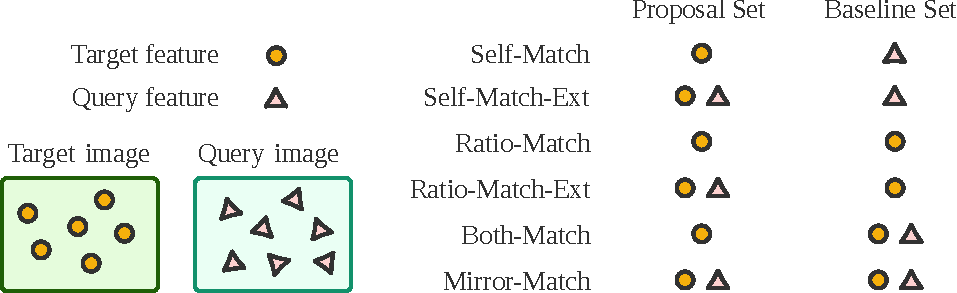
\includegraphics[width=0.95\columnwidth]{images/overview-wide}
\caption{Graphical representation of the \emph{Baseline} and 
\emph{Proposal Set} for different methods in the proposed framework}
\label{fig:overview}
\end{figure}

Given two images we can construct the proposal and baseline sets in six different ways as illustrated in Figure~\ref{fig:overview}. In the case of \emph{Ratio-Match} \cite{lowe2004sift} the \emph{proposal set} consists of all the feature points in the \emph{target image}.  Similarly the \emph{baseline set} consists of all the feature points in the \emph{target image} except the \emph{proposed} match. For \emph{Ratio-Match} this practically means that given a query feature, $f_q$, the \emph{proposed match} and the \emph{baseline match} are the two nearest neighbors in the set of feature points in the \emph{target image}, and the ratio is decided uniquely based on the \emph{target image}. In turn \emph{Mirror-Match} as introduced by the authors in \cite{arnfred2013mirror} works by constructing the \emph{proposal set} and \emph{baseline set} by combining features from both the \emph{query} and \emph{target image}. By similar variations of the \emph{proposal} and \emph{baseline set} we derive four more algorithms as illustrated in Figure~\ref{fig:overview}. We will not discuss \emph{Self-Match-Ext} and \emph{Both-Match} further in this paper since we prove them to be equivalent with \emph{Self-Match} and \emph{Mirror-Match} respectively in \ref{A:self} and \ref{A:mirror}.

\begin{algorithm}[htb]
\caption{Generalized matching algorithm for two images}
\label{alg-gen}
\begin{algorithmic}
    \Require $I_{query}, I_{target}$ : images, $\tau \in [0,1]$
    \State $F_{q} = get\_features(I_{query})$
    \State $F_{t} = get\_features(I_{target})$
\State $F_{proposal-all} = get\_proposal\_features(F_{q}, 
F_{t})$
\State $F_{baseline-all} = get\_baseline\_features(F_{q}, 
F_{t})$
\State $M = \varnothing$
\ForAll{$f_q \in F_{q}$}
    \State $F_{proposal} = F_{proposal-all} \setminus 
    \left\{f_q\right\}$
    \State $f_p \gets getNearestNeighbo\text{r}(f_q, F_{proposal})$
    \State $F_{b} = F_{baseline-all} \setminus \left\{f_q, 
    f_p\right\}$
    \State $f_b \gets getNearestNeighbo\text{r}(f_q, F_{b})$
    \State $r \gets distance(f_q, f_p) / distance(f_q, f_b)$
    \If{$(r < \tau) \wedge (f_p \in F_{t})$}
        \State $matches \gets matches \cup \left(f_q, f_p\right)$
	\EndIf
\EndFor \\
\Return $M$
\end{algorithmic}
\end{algorithm}

Algorithm~\ref{alg-gen} shows the generalized matching framework where the \emph{proposal set} and \emph{baseline set} are defined according to Figure~\ref{fig:overview}.  In practice for e.g.\ \emph{Ratio-Match} we can obtain $f_p$ and $f_b$ by finding the two nearest neighbors of $F_{t}$. The other algorithms can be optimized similarly. Figure~\ref{fig:matching} illustrates the structure of this algorithm.


\begin{figure}[htb]
\centering
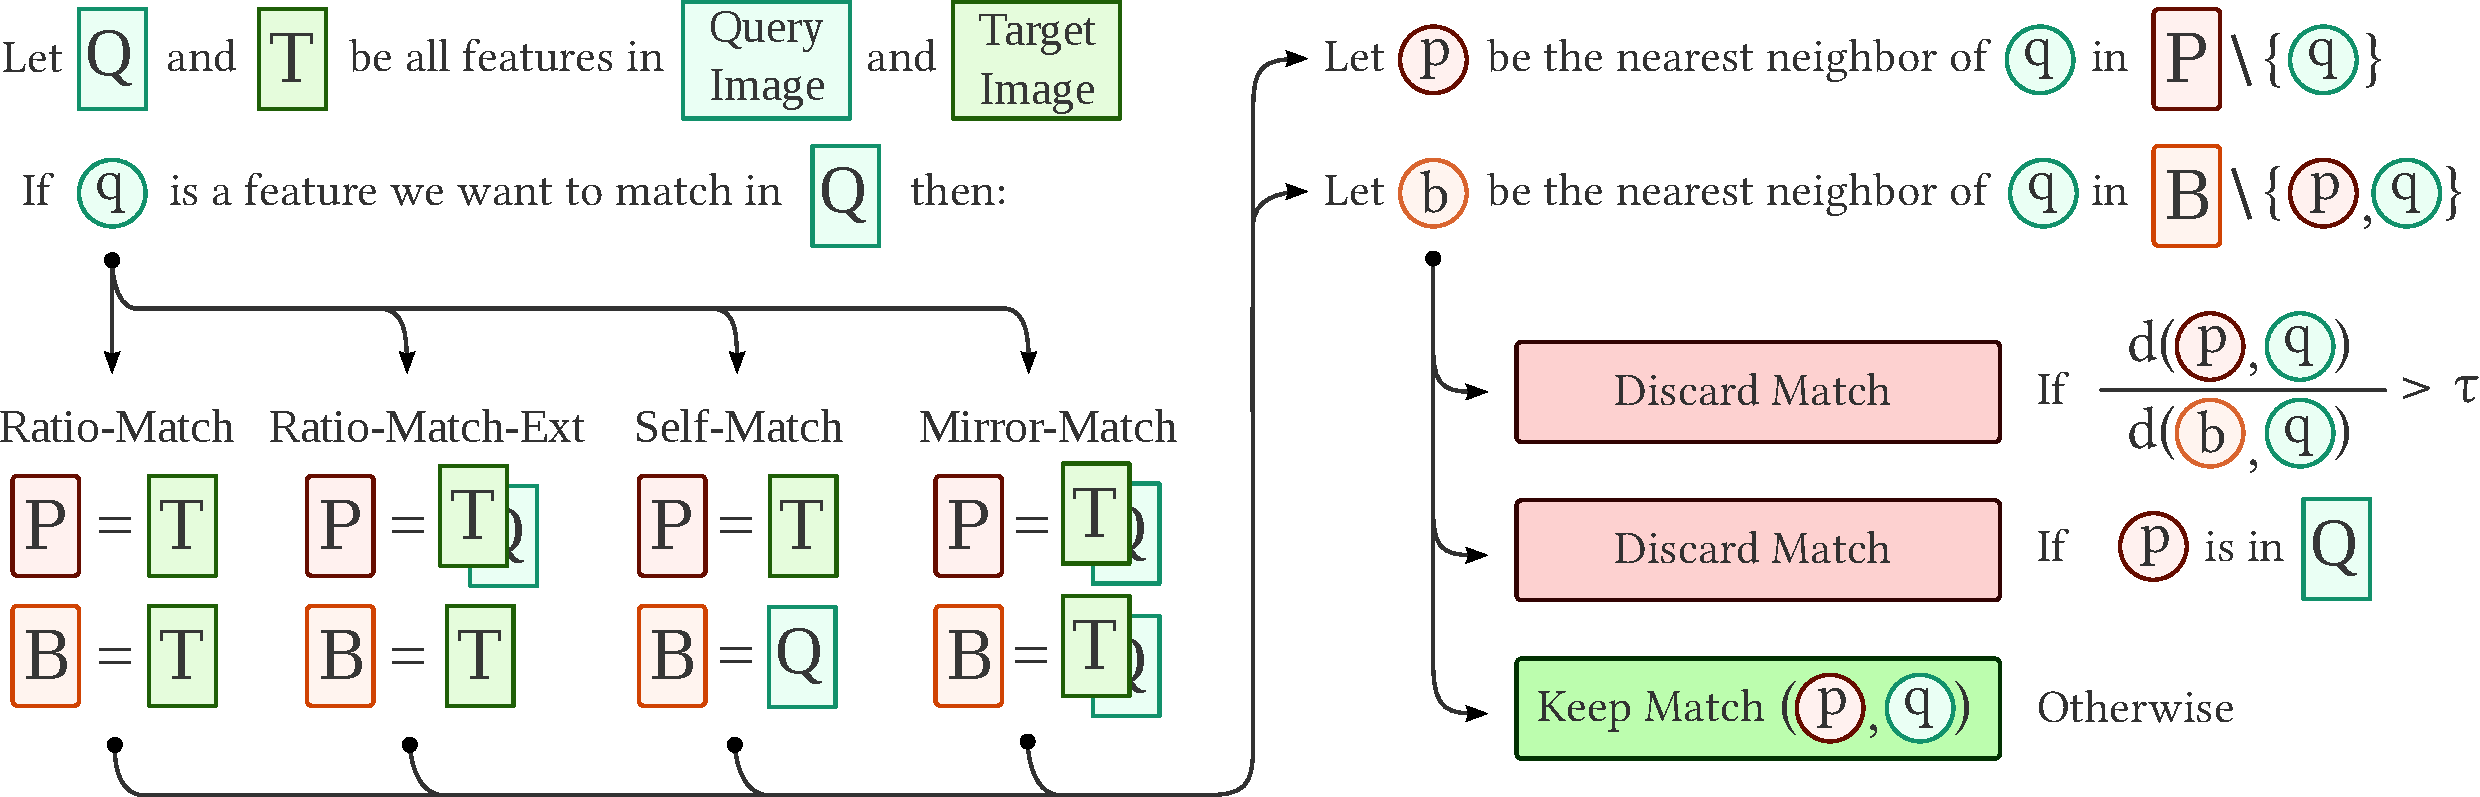
\includegraphics[width=\columnwidth]{images/matching-wide}
\caption{Feature matching flow chart. $\tau$ 
is the ratio threshold, and $d(x,y)$ is the distance between two feature 
descriptors $x$ and $y$.}
\label{fig:matching}
\end{figure}
%

For some methods it is possible that the \emph{proposal match} is a feature from the \emph{query image}, in which case we discard the match as an untrue correspondence.  It also happens that we encounter correspondences with $r>1$, in which case the match is also discarded.  Take for example the case of \emph{Self-Match} where we might find that the nearest neighbor of a feature in the \emph{target image} is further from the query feature than the nearest neighbor in the \emph{query image}. In this case the match is discarded. 

%
\subsection{Uniqueness Ratio}
%

The main distinguishing factor between the algorithms in the framework is the final ratio between the distance of the two nearest neighbors of a query feature which decides if we keep or discard a match. We illustrate this process in Figure~\ref{fig:matching}.

We can define a calculation of this ratio that is common to all algorithms in the framework, which allows us to compare the algorithms theoretically. To do so we we introduce the \emph{uniqueness ratio} $r$, based on the concept of a nearest neighbor.

Given a feature $f_i$ and a set of features $F$, the nearest neighbor of $f_i$ in $F$ is calculated as follows: 
\begin{equation*}
\argmin_{f_j \in F} d(f_i, f_j)
\end{equation*}
Here, $d(f_i, f_j)$ is the distance between feature descriptors.With SIFT and SURF this is the Euclidean distance of the feature vectors \cite{lowe2004sift,bay2006surf}, whereas BRIEF, BRISK, and FREAK use the Hamming distance \cite{leutenegger2011brisk,calonder2010brief,alahi2012freak}.  

If we let $f_p \in F_{p}$ and $f_b \in F_{b}$ be the nearest neighbors of a feature $f_q$ in $F_{p}$ and $F_{b}$, the \emph{uniqueness ratio} is defined as follows:
\begin{align*}
    r &= \text{r}(f_{q}, F_{p}, F_{b}) \\
        &= \frac{d(f_{q}, f_{p})}{d(f_{q}, f_{b})}.
\end{align*}

The performance in terms of precision and recall of any algorithm from the proposed framework is uniquely identified by the \emph{uniqueness ratio} $r$. To show this we let $K$ be the number of possible true correspondences between \emph{query} and \emph{target image}. \emph{Precision} and \emph{recall} are defined as:
\begin{align*}
    \textrm{Recall} &= \frac{\#\textrm{Correct}}{K} \\
    \textrm{Precision} &= \frac{\#\textrm{Correct}}{\#\textrm{Correct} + \#\textrm{Incorrect}}
\end{align*}
Given $f_{p} \in F_{p}$ as the nearest neighbor of some $f_q \in F_{q}$, we define the set of features $F_{true}$ as $\left\{ f_{q} \in F_{q} \mid f_{p} \text{ is a true correspondence of } f_{q} \right\}$ and $F_{false}$ as $F_{q} \setminus F_{true}$.  We can then define the number of correct and incorrect matches as follows:
\begin{align*}
    \textrm{keep\_match}(f_{q}) &= \twopartdef{ 1 }{\text{r}(f_{q}, 
    F_{p}, F_{b}) <
    \tau}{0}{\textrm{otherwise}} \\
    \#\textrm{Correct} &= \sum_{f_{q} \in F_{true}} 
    \textrm{keep\_match}(f_{q})\\
    %\mathbbm{1}_{\left\{ \right\}} \\
    \#\textrm{Incorrect} &= \sum_{f_{q} \in F_{false}}
    \textrm{keep\_match}(f_{q})
    %\mathbbm{1}_{\left\{ r < \tau\right\}}
\end{align*}
If for every query feature $f_{q}$, $r$ is identical across two matching methods, then they return identical results. 

\subsection{Proofs of Algorithm Performance}
\label{S:Proofs}

Under the following three assumptions, which largely reflect the performance of matching feature points in practice, we can theoretically compare the performance of the different algorithms shown in Figure~\ref{fig:overview}:

\begin{enumerate}
    \item{For a query and \emph{target image} we assume that for any point in 
        the \emph{query image} there is at most one real correspondence in the 
    \emph{target image} and no real correspondences in the \emph{query image} itself 
as assumed by \emph{Ratio-Match}.}
    \item{We assume that distances of feature descriptors are well 
            behaved.  More precisely, given $f_q$, a feature from the 
            \emph{query image}, and $f_{match}$, the real correspondence 
            from the set of features in the \emph{target image} 
            $F_{t}$, we assume $\forall f_i \in F_{proposal}, 
            f_i \neq f_{match}: d(f_q,f_{match}) < d(f_q, f_i)$.}
    %\item{We assume that features within one image resemble each other 
            %more than features in different images. That is, given 
            %$f_a,
    %        f_i \in F_1$ and $f_b, f_j \in F_2$ where $(f_i, f_j)$ and 
    %    $(f_a, f_b)$ are true correspondences, and $F_1$ and $F_2$ are 
    %features collected from different images then we expect that 
            %$d(f_a, f_i)% < d(f_a, f_j)$ and $d(f_b, f_j) < d(f_b, 
            %f_i)$}
     \item{For a set of query features $F_{q}$ with a true 
             correspondence in the \emph{target image}, we assume that 
             the distribution of \emph{uniqueness ratios} using $F_{t}$ as 
             the baseline set is similar to using $F_{q}$, since the 
         two images in the case of true correspondences are bound 
     to share part of the same scene.}
    \end{enumerate}

Based on these assumptions we prove that \emph{Ratio-Match-Ext} is equal or better than \emph{Ratio-Match} in terms both precision and recall.  Consider the nearest neighbor $f_{p}$ of a query feature $f_{q}$ and the two cases where we either have the $f_{p} \in F_{q}$ or $f_{p} \in F_{t}$. For $f_{p} \in F_{t}$ the uniqueness ratio of \emph{Ratio-Match-Ext} is:
\begin{align*}
    r &= \text{r}(f_{q}, F_{p}, F_{b}) \\
        &= \text{r}(f_{q}, F_{q} \cup F_{t}, F_{b})\\
        &= \text{r}(f_{q}, F_{t}, F_{b})
\end{align*}
Since $F_{p} = F_{t}$ for \emph{Ratio-Match} this shows that when the nearest neighbor is found in the \emph{target image}, the two algorithms behave identically. For $f_{p} \in F_{q}$ \emph{Ratio-Match} gives us the following ratio:
\begin{align*}
    r &= \text{r}(f_{q}, F_{p}, F_{b}) \\
        &= \text{r}(f_{q}, F_{t}, F_{t}).
\end{align*}

That is, \emph{Ratio-Match} calculates the ratio based on the two nearest correspondences in the \emph{target image}. \emph{Ratio-Match-Ext} on the other hand does not return any correspondence because the nearest neighbor is in the \emph{query image}. Since query features with a nearest neighbor in the \emph{query image} are false correspondences per assumption \#1 and \#2, this proves that \emph{Ratio-Match-Ext} has superior \emph{Precision} to \emph{Ratio-Match} while maintaining equal \emph{Recall}.

Next we show that \emph{Mirror-Match} is equal or better than \emph{Ratio-Match-Ext} in terms of precision and recall. Consider as before the nearest neighbor $f_{p}$ of a query feature $f_{q}$. When $f_{p}$ resides in the \emph{query image} both algorithms behave alike and discard the match.  However, consider the uniqueness ratio of \emph{Mirror-Match} for the case where $f_{p}$ resides in the \emph{target image}:
\begin{align*}
    r &= \text{r}(f_{q}, F_{p}, F_{b}) \\
        &= \text{r}(f_{q}, F_{p}, F_{q} \cup F_{t})\\
        &= \max( \text{r}(f_{q}, F_{p}, F_{t}), 
    \text{r}(f_{q}, F_{p}, F_{q}) ).
\end{align*}
For a true correspondence the \emph{uniqueness ratio} using $F_{q}$ as a baseline is distributed similarly to the ratio when using $F_{t}$ according to assumption \#3. In this case the algorithm performs like \emph{Ratio-Match-Ext}.  However, for an untrue correspondence with a baseline match in the \emph{query image} which is closer than the baseline match in the \emph{target image}, \emph{Mirror Match} will return a worse \emph{uniqueness ratio}. This in turns means that \emph{Mirror Match} is equal or better than \emph{Ratio-Match-Ext} in terms of  \emph{Precision} while maintaining equal \emph{Recall}.

Using a similar procedure we can prove that \emph{Self-Match} is equal to \emph{Self-Match-Ext} and \emph{Both-Match} is equal to \emph{Mirror Match}.  The details can be found in \ref{A:self} and \ref{A:mirror}, respectively.

We have thus proven that -- based on assumptions \#1-3 -- for any given recall rate, the precision of the algorithms in the framework compares as follows: 
\begin{align*}
    \textit{Ratio-Match} &\leq \textit{Ratio-Match-Ext} \leq 
    \textit{Mirror-Match}
\end{align*}

\emph{Self-Match} is most closely related to \emph{Ratio-Match} in that both the \emph{baseline} and \emph{proposal} set are created based on only one image. While the \emph{proposal set} for both algorithms is based on the \emph{target image}, \emph{Self-Match} uses the \emph{query image} for the \emph{baseline set} while \emph{Ratio-Match} sticks with the \emph{target image}. For cases where there is a lot of overlap in between the \emph{target} and \emph{query image} they should perform similarly. However when we match images where the \emph{target image} may not overlap at all with the \emph{query image}, using the \emph{query image} and not the \emph{target image} as a \emph{baseline set} seems like a reasonable choice given that the baseline set in this case would be closer to the feature matched and more strictly rule out untrue correspondences.

\subsection{Discussion of Assumptions}
\label{ref:disc_assumptions}

% Assumption 1
%For a query and \emph{target image} we assume that for any point in the query 
%image there is at most one real correspondence in the \emph{target image} and 
%no real correspondences in the \emph{query image} itself as assumed by 
%\emph{Ratio-Match}

% Assumption 2
%We assume the distances of feature descriptors behave in a \emph{nice} 
%manner. That is, given $f_q$, a feature from the \emph{query image} and 
%$f_{match}$, the real correspondence from the set of features in the 
%\emph{target image} $F_{t}$, we have that $\forall f_i \in 
%F_{proposal}, f_i \neq f_{match}: d(f_q,f_{match}) < d(f_q, f_i)$

% Assumption 3
%For a query feature, $f_q$ with a true correspondence in the 
%\emph{target image}, we assume that the \emph{uniqueness ratio} using 
%$F_{t}$ is similar to the \emph{uniqueness ratio} using $F_{q}$, 
%since the two images in this case are guaranteed to share part of the 
%same scene

The three assumptions underlying the formal ranking of algorithms presented above have been chosen to reflect conditions under which we would ideally match feature points. However, for each assumption there exist corner cases where it is no longer valid. In this section we discuss these corner cases in order to review the circumstances under which the absolute or relative performance of the algorithms might differ.

The first assumption states that there is at most one unique match to every feature point, which is often the case for natural images. However, for the recognition of object classes or in images with repetitive content, a point in the \emph{query image} might have several true correspondences in the \emph{target image}, so using a \emph{baseline match} from the \emph{target image} will lead to a much higher \emph{uniqueness ratio}. However, as long as the \emph{query image} does not contain repetitive objects, we can still use \emph{Self-Match} without loss of precision.

According to the second assumption, feature descriptors behave such that when matched, a true correspondence to a query feature will always be the nearest neighbor. For practical implementations of feature detectors and descriptors, this property strongly depends on the differences between \emph{query} and \emph{target image}, as shown in  \cite{mikolajczyk2005performance,tuytelaars2008local}. In the degenerate case where the closest match is not an actual correspondence, there is no reason why this match should be disproportionately closer to the \emph{query feature} than any matches in the \emph{target image}, so in most cases we would expect the \emph{uniqueness ratio} to be high (signifying a bad match). This means that with a lenient threshold (close to 1), the guarantees about precision and recall equivalence between the different ratio algorithms might no longer hold due to the inconsistent descriptor behavior. It is worth noting that if assumption \#2 holds, matching using only nearest neighbor is not necessarily optimal, unless there is a complete scene overlap between the images matched. For cases where there is little or no overlap, a nearest neighbor would indiscriminately return false matches even with well-behaved feature descriptors.

The third assumption states that the \emph{uniqueness ratios} using either the \emph{query} or \emph{target image} as the baseline set would be similar in distribution given that the feature point we are matching has a true correspondence. We can support this assumption by looking at the \emph{uniqueness ratios} returned by \emph{Self-Match} and \emph{Ratio-Match}, since they use the \emph{query} and \emph{target image} respectively to calculate the \emph{uniqueness ratio}.  Figure~\ref{fig:ratio_hist} shows the actual \emph{uniqueness ratios} measured from 3024 image pairs featuring 3D objects (see below for more on this dataset).  For ratios lower than $0.7$, the \emph{uniqueness ratios} are similar, but as we approach more lenient thresholds, the ratios based on the \emph{query image} are higher than those for the \emph{target image}. This means that the third assumption is invalid for more lenient thresholds, and we can no longer expect \emph{Mirror-Match} to outperform \emph{Ratio-Match-Ext} in terms of precision without a penalty in recall.


\begin{figure}[htb]
\centering
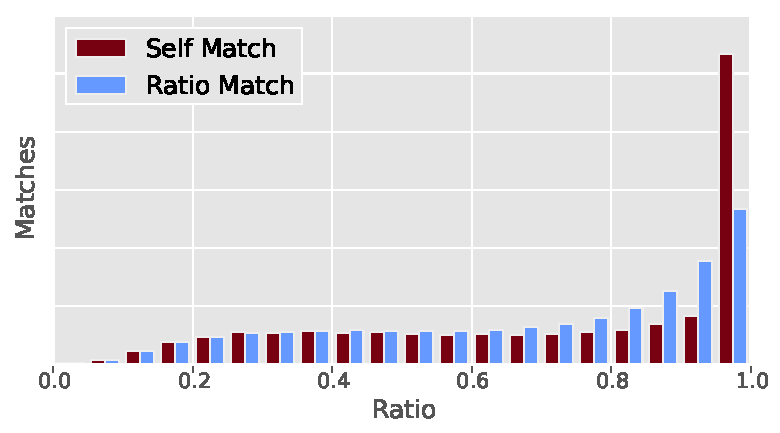
\includegraphics[width=0.7\columnwidth]{images/results_ratio_hist}
\caption{Normalized histogram of the \emph{uniqueness ratios} of true 
correspondences for 3000 image pairs.}
\label{fig:ratio_hist}
\end{figure}


\section{Experiments and Results}
\label{S:Experiments}
%
In this section we present the experiments and evaluation results comparing \emph{Self-Match}, \emph{Ratio-Match}, \emph{Ratio-Match-Ext} and \emph{Mirror-Match}. 

We evaluate the algorithm on the 3D Objects database released by Moreels and Pietro \cite{moreels2007evaluation} in Section~\ref{S:3dobjects}. This database contains a set of 86 3D objects photographed from all sides at 5 degree intervals from two different elevation angles and under three different lighting conditions. 

For the experiments we use the SIFT descriptor and keypoint detector with default parameters as implemented in the OpenCV library 2.4.6.  To further test how the framework performs across descriptors, we evaluate SURF \cite{bay2006surf}, BRISK \cite{leutenegger2011brisk}, BRIEF \cite{calonder2010brief}, and FREAK \cite{alahi2012freak} in Section~\ref{label:desc}. 

Across all experiments, only the luminance channel is used in the feature detection and description stage.  Images larger than $1024\!\times\!768$ are resized to fit within those dimensions using ImageMagick with default parameters.  

\subsection{Evaluation of Methods}
\label{S:3dobjects}

The 3D objects dataset by Moreels and Pietro \cite{moreels2007evaluation} allows us to experimentally compare matching algorithms over a large range of object and surface types rotated on a turnstile and photographed from every 5 degree turn.  15 objects from the dataset are shown in Figure~\ref{fig:3d_objects}.  We use images of 84 different objects under three different lighting conditions at 12 different angle intervals, conducting experiments with a total of 3024 image pairs.  

\begin{figure}[htb]
    \centering
    \begin{subfigure}[t]{0.15\columnwidth}
        \centering
        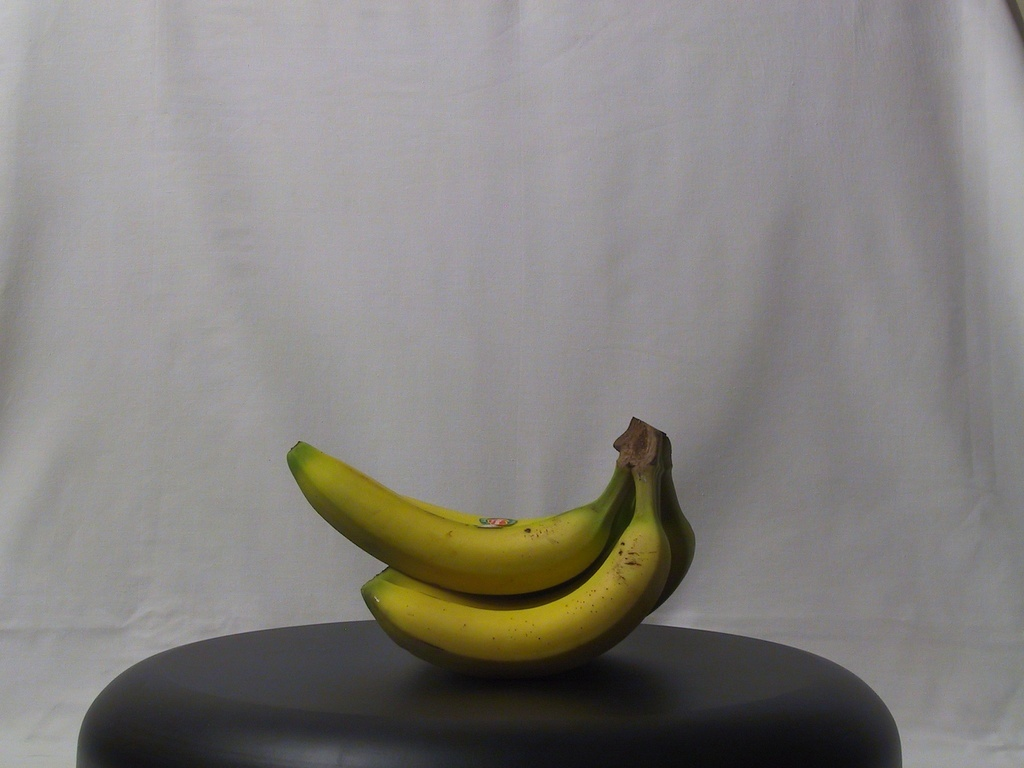
\includegraphics[width=1\columnwidth]{images/3d/1}
    \end{subfigure}%
    ~ %
    \begin{subfigure}[t]{0.15\columnwidth}
        \centering
        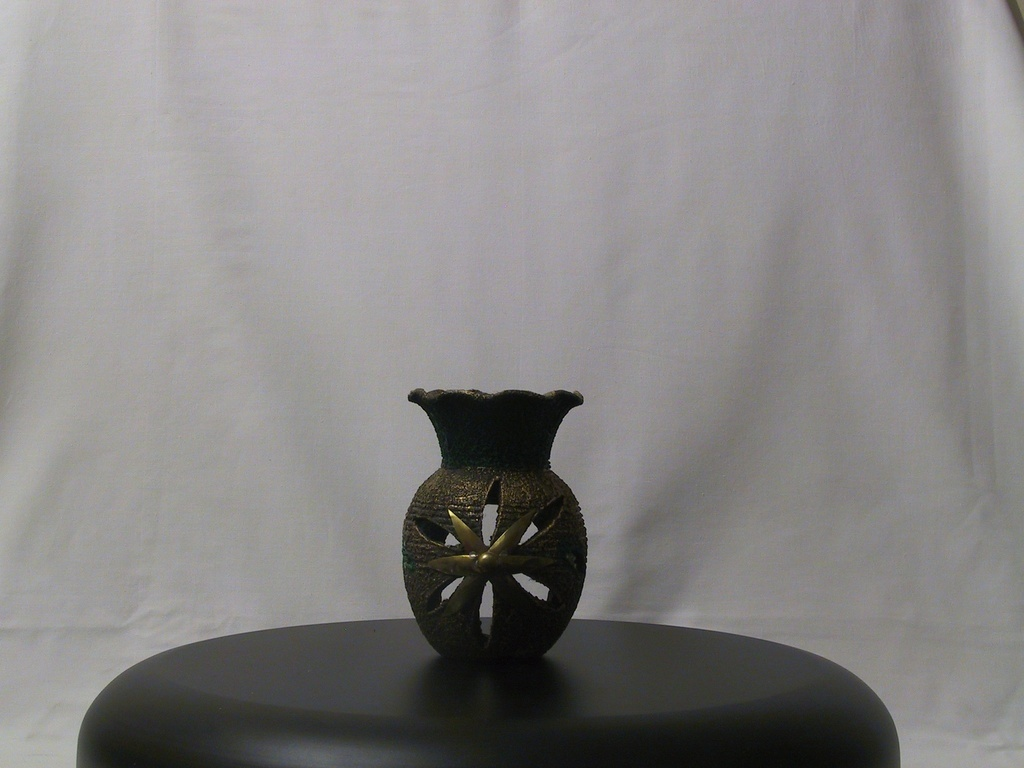
\includegraphics[width=1\columnwidth]{images/3d/2}
    \end{subfigure}%
    ~ %
    \begin{subfigure}[t]{0.15\columnwidth}
        \centering
        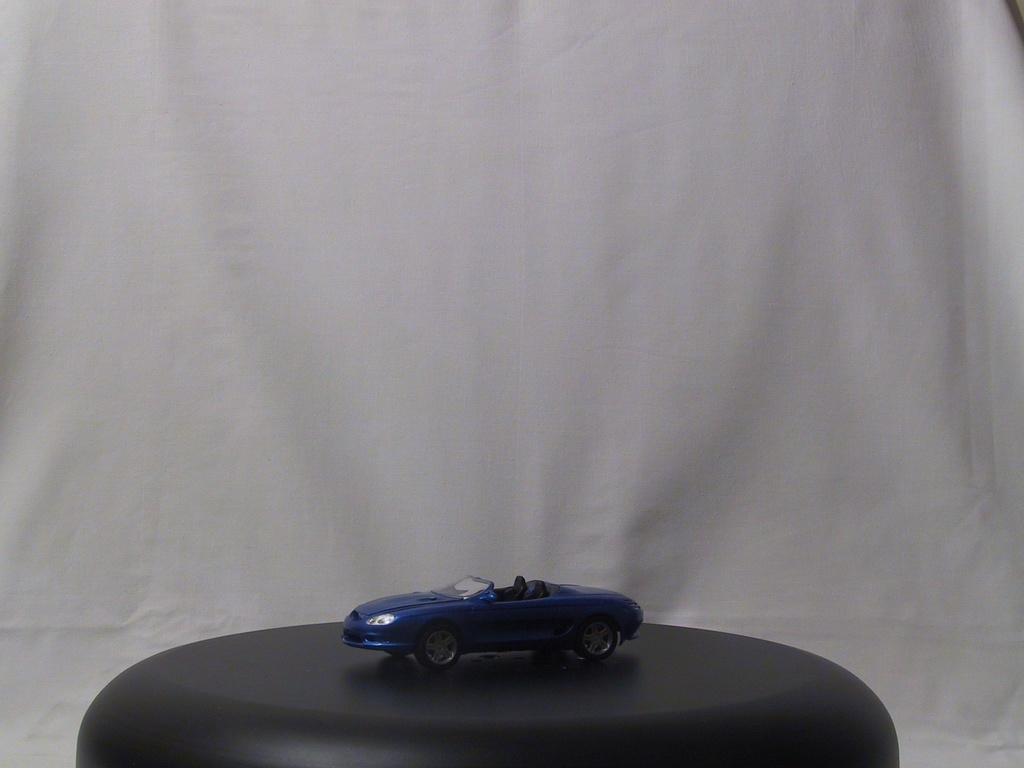
\includegraphics[width=1\columnwidth]{images/3d/3}
    \end{subfigure}%
    ~ %
    \begin{subfigure}[t]{0.15\columnwidth}
        \centering
        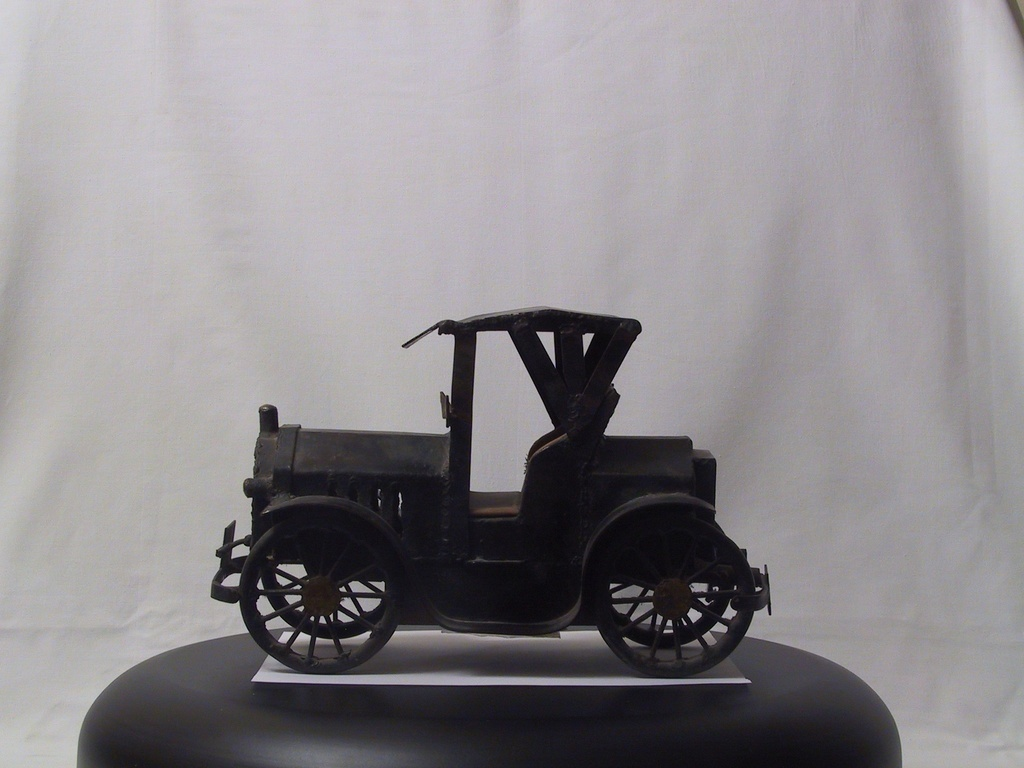
\includegraphics[width=1\columnwidth]{images/3d/4}
    \end{subfigure}%
    ~ %
    \begin{subfigure}[t]{0.15\columnwidth}
        \centering
        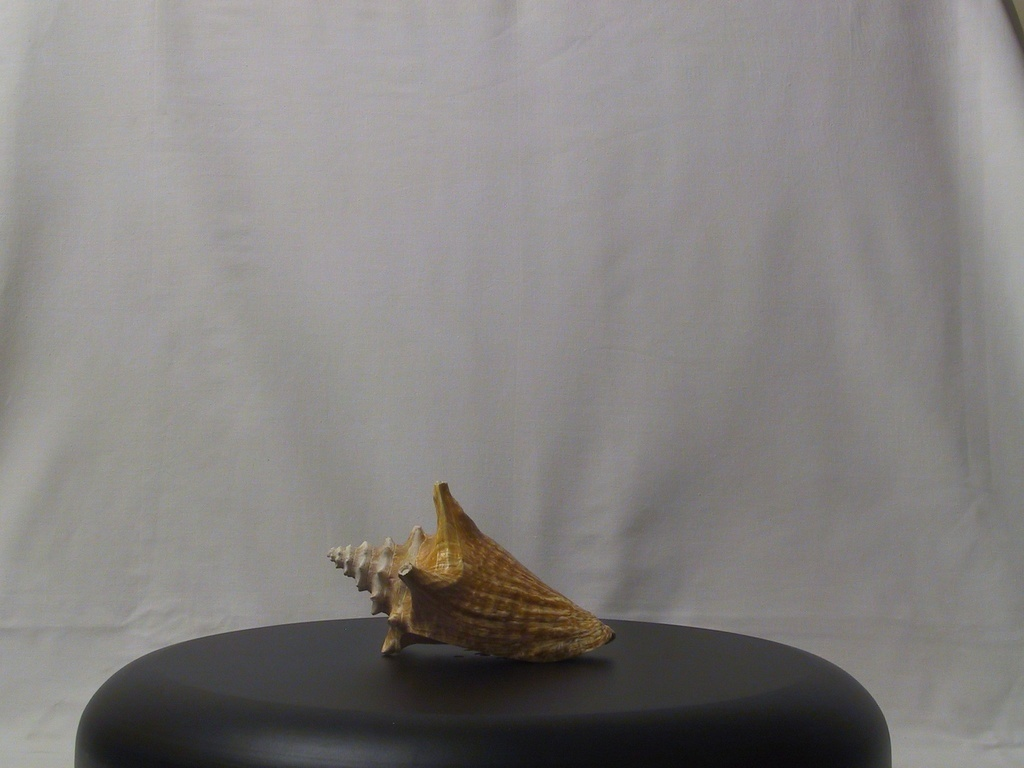
\includegraphics[width=1\columnwidth]{images/3d/5}
    \end{subfigure}%
    \vspace{1.5 mm}

    \begin{subfigure}[t]{0.15\columnwidth}
        \centering
        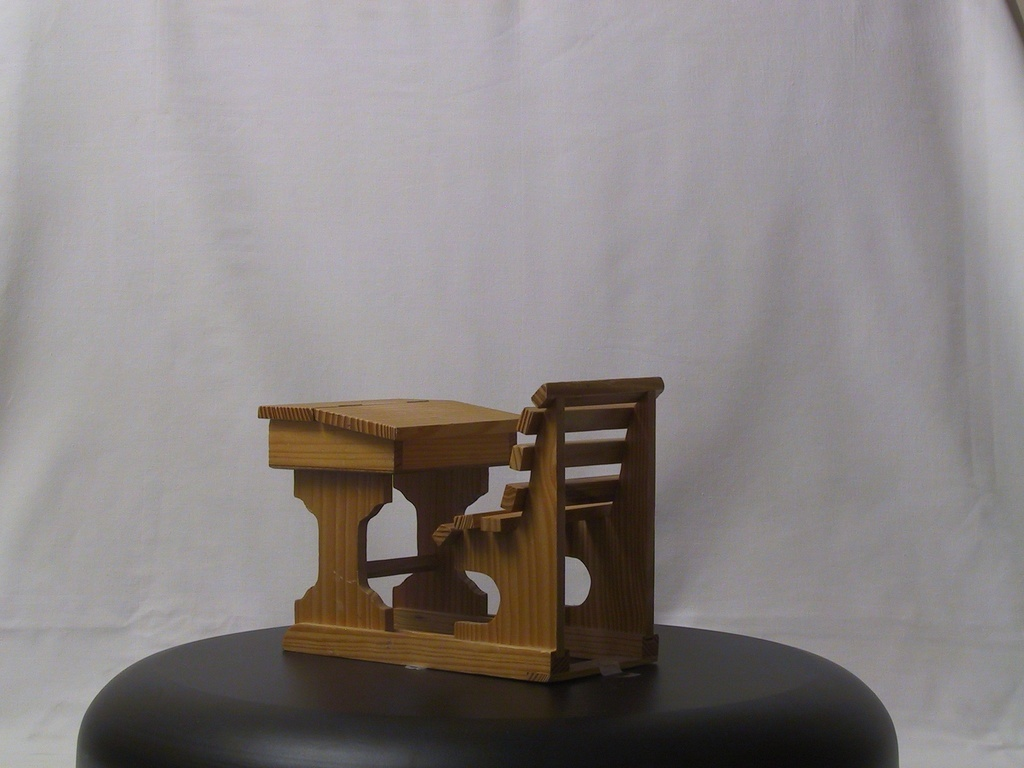
\includegraphics[width=1\columnwidth]{images/3d/6}
    \end{subfigure}%
    ~ %
    \begin{subfigure}[t]{0.15\columnwidth}
        \centering
        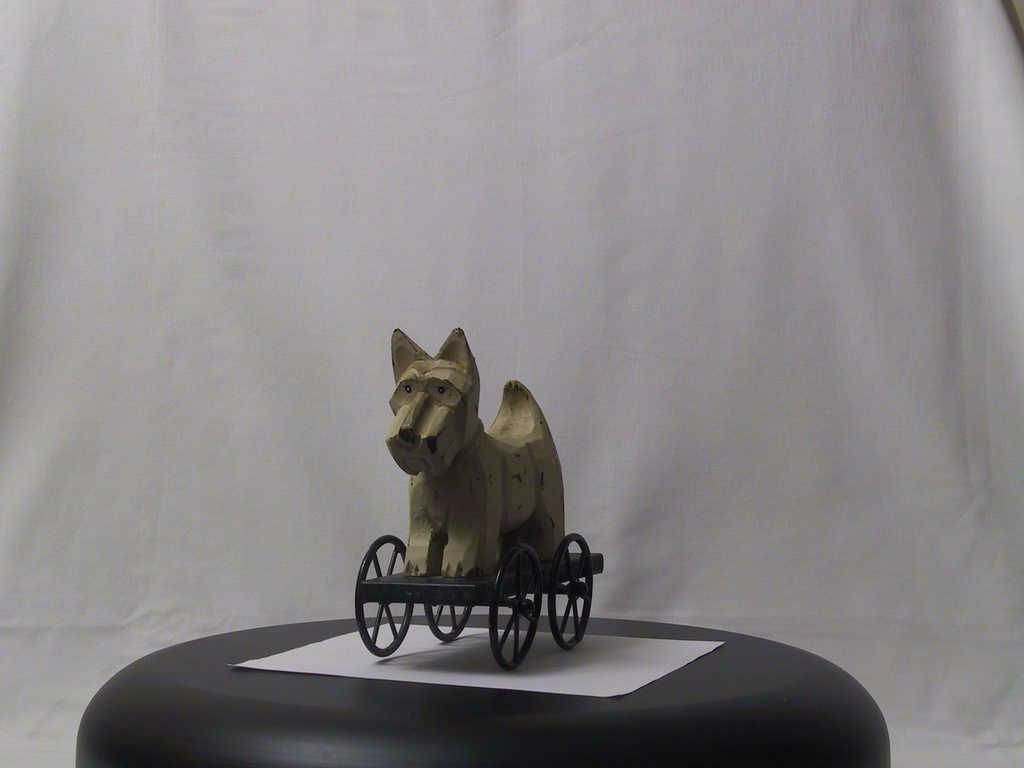
\includegraphics[width=1\columnwidth]{images/3d/7}
    \end{subfigure}%
    ~ %
    \begin{subfigure}[t]{0.15\columnwidth}
        \centering
        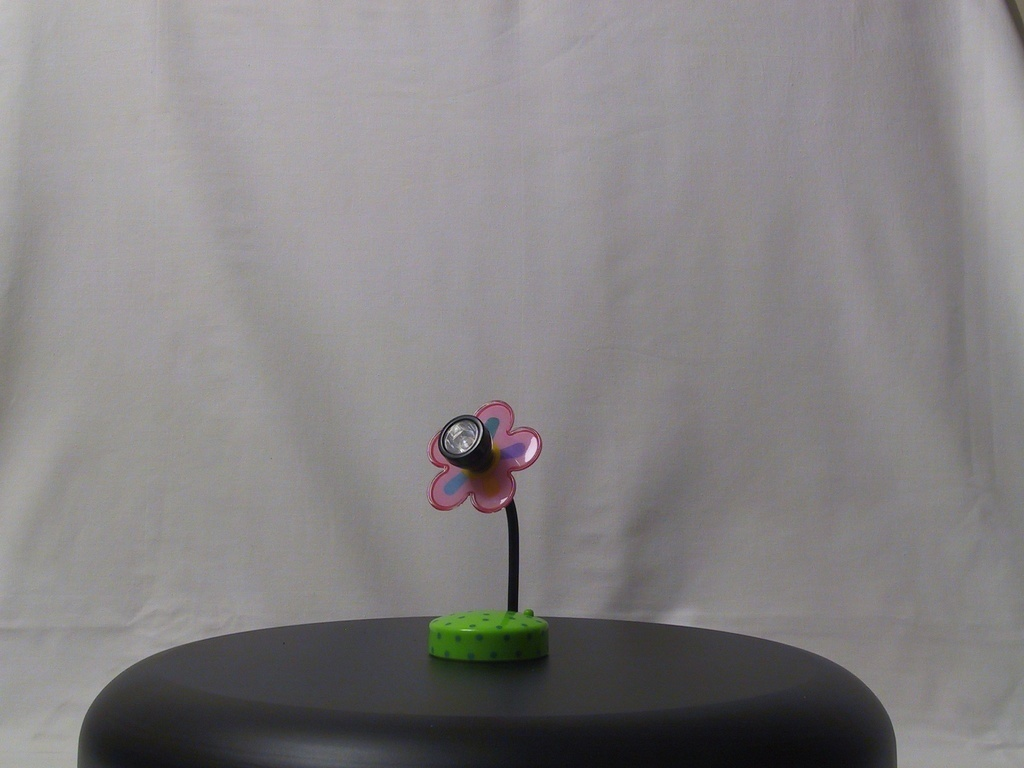
\includegraphics[width=1\columnwidth]{images/3d/8}
    \end{subfigure}%
    ~ %
    \begin{subfigure}[t]{0.15\columnwidth}
        \centering
        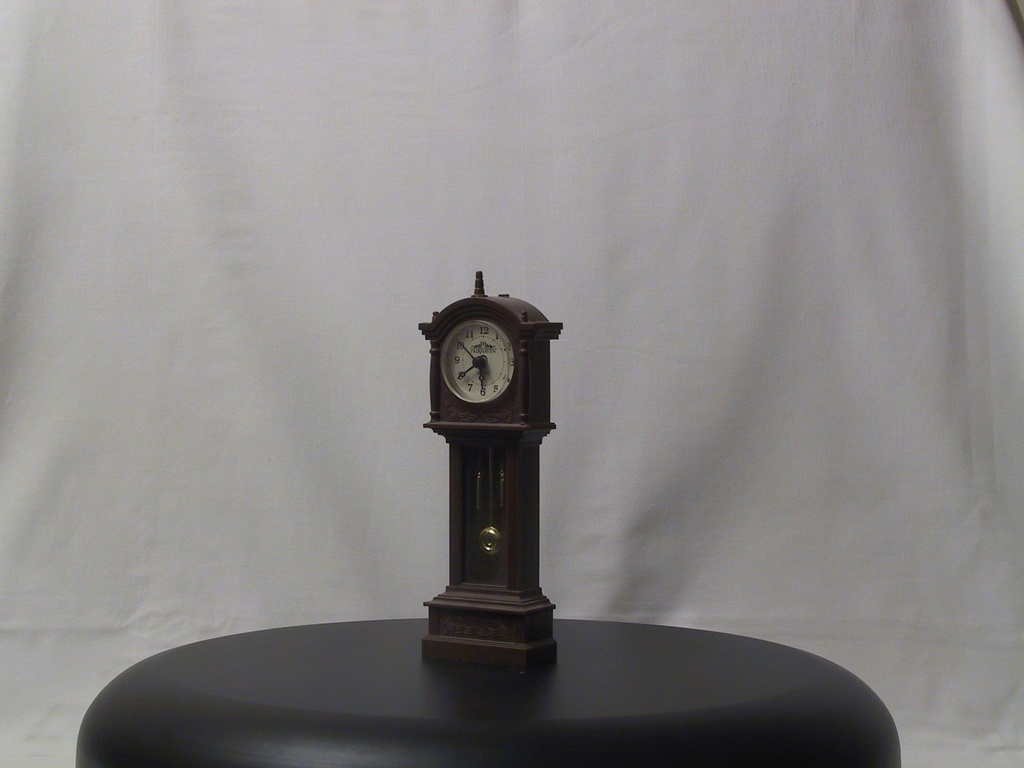
\includegraphics[width=1\columnwidth]{images/3d/9}
    \end{subfigure}%
    ~ %
    \begin{subfigure}[t]{0.15\columnwidth}
        \centering
        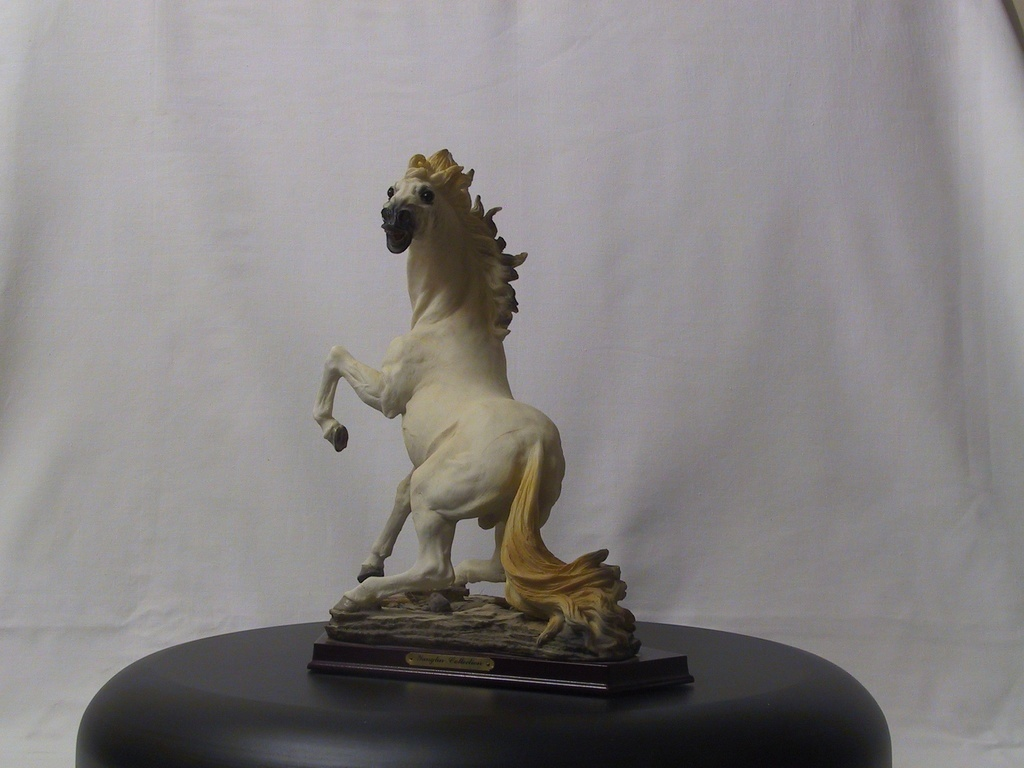
\includegraphics[width=1\columnwidth]{images/3d/10}
    \end{subfigure}%
    \vspace{1.5 mm}

    \begin{subfigure}[t]{0.15\columnwidth}
        \centering
        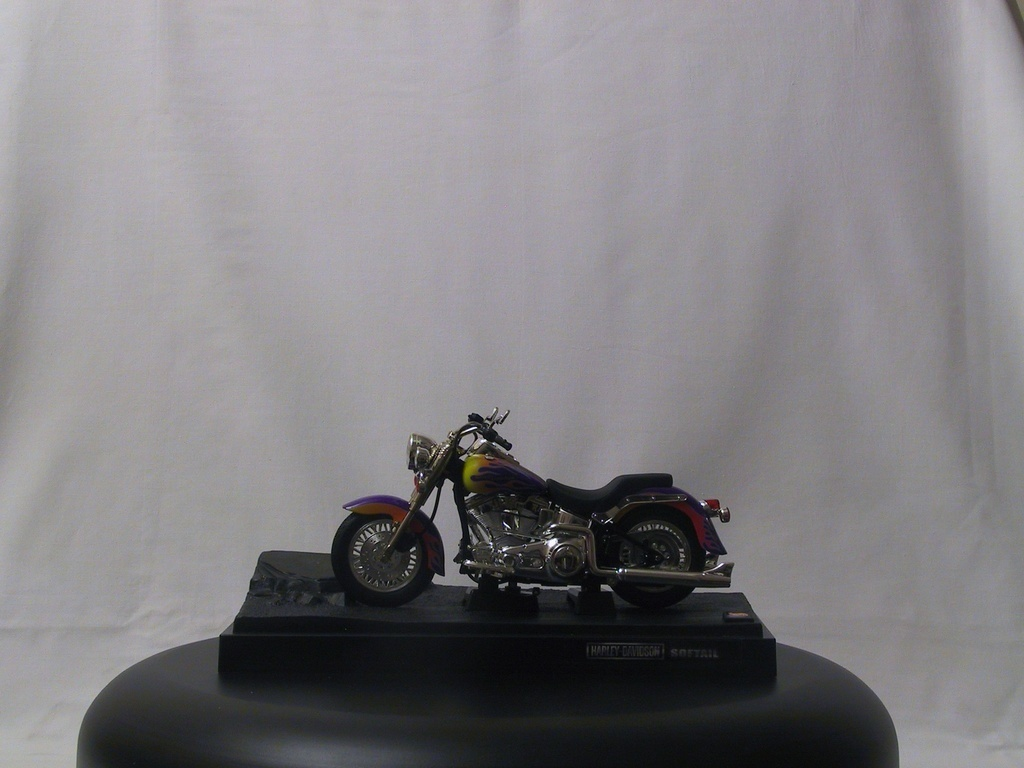
\includegraphics[width=1\columnwidth]{images/3d/11}
    \end{subfigure}%
    ~ %
    \begin{subfigure}[t]{0.15\columnwidth}
        \centering
        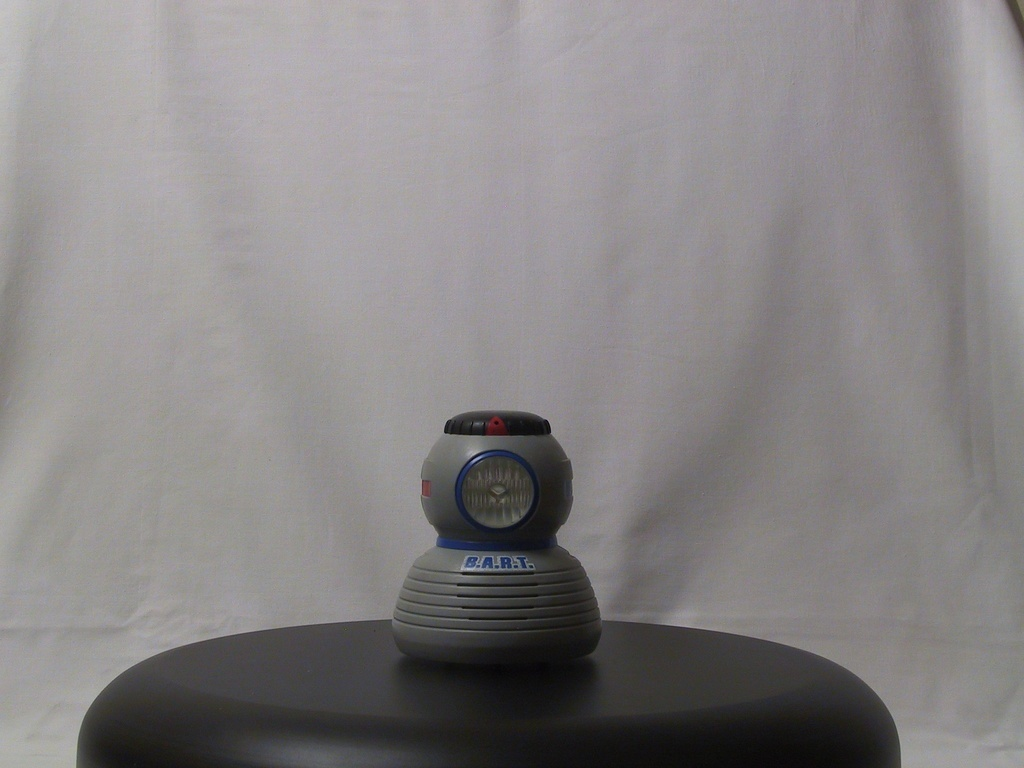
\includegraphics[width=1\columnwidth]{images/3d/12}
    \end{subfigure}%
    ~ %
    \begin{subfigure}[t]{0.15\columnwidth}
        \centering
        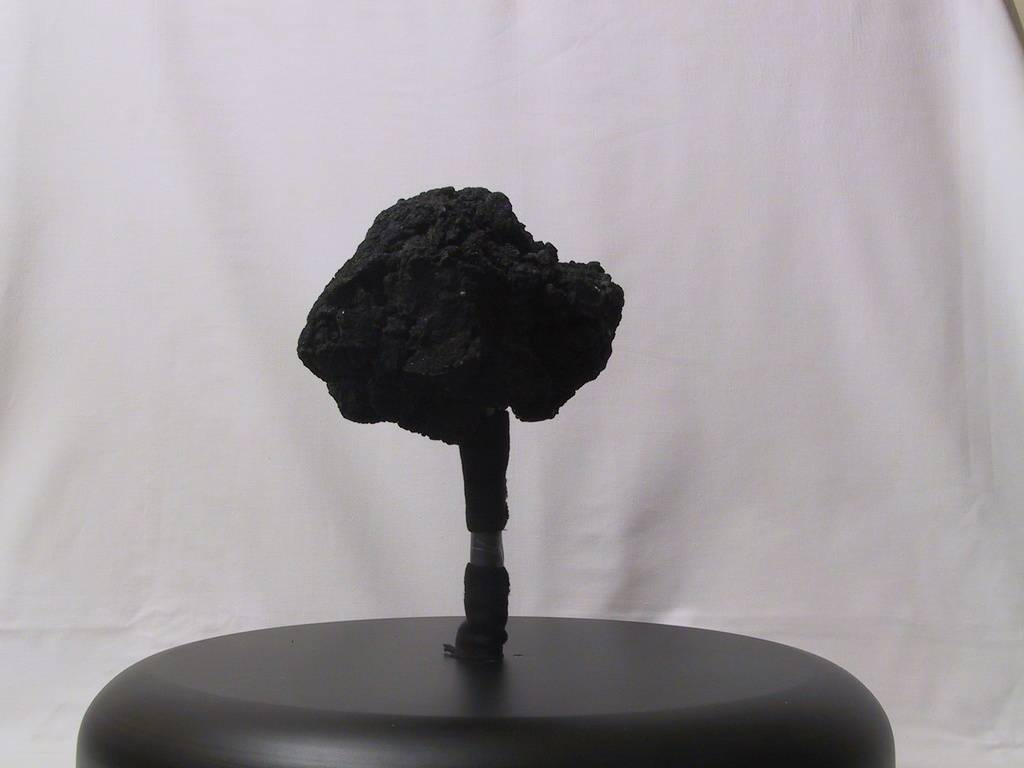
\includegraphics[width=1\columnwidth]{images/3d/13}
    \end{subfigure}%
    ~ %
    \begin{subfigure}[t]{0.15\columnwidth}
        \centering
        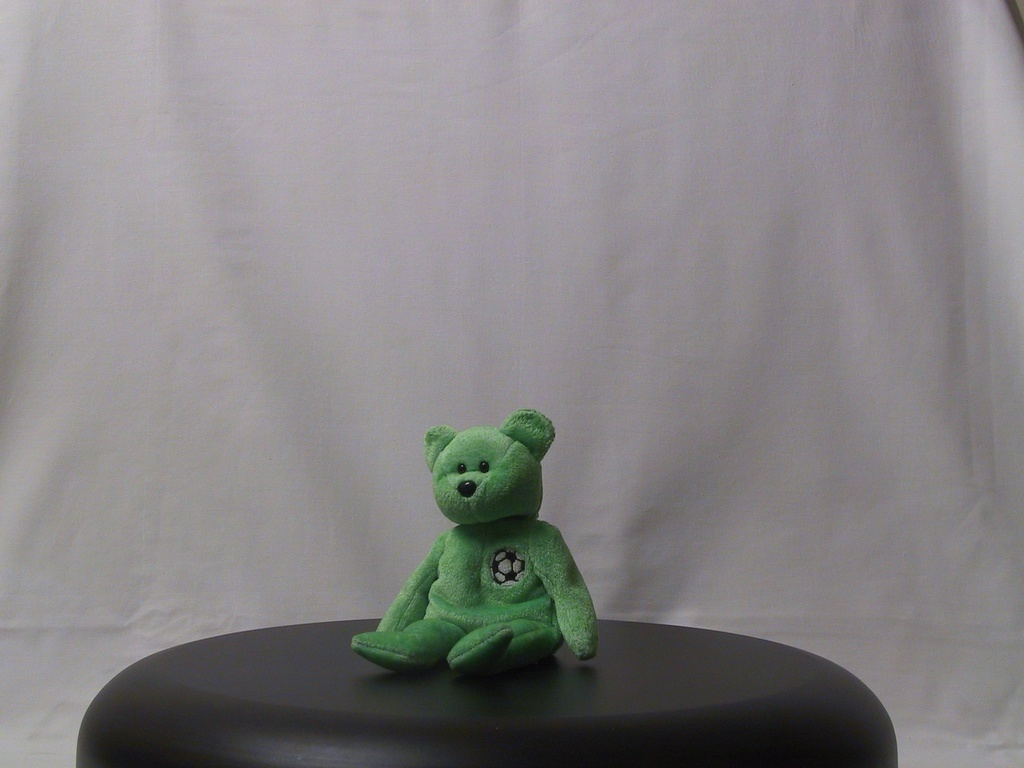
\includegraphics[width=1\columnwidth]{images/3d/14}
    \end{subfigure}%
    ~ %
    \begin{subfigure}[t]{0.15\columnwidth}
        \centering
        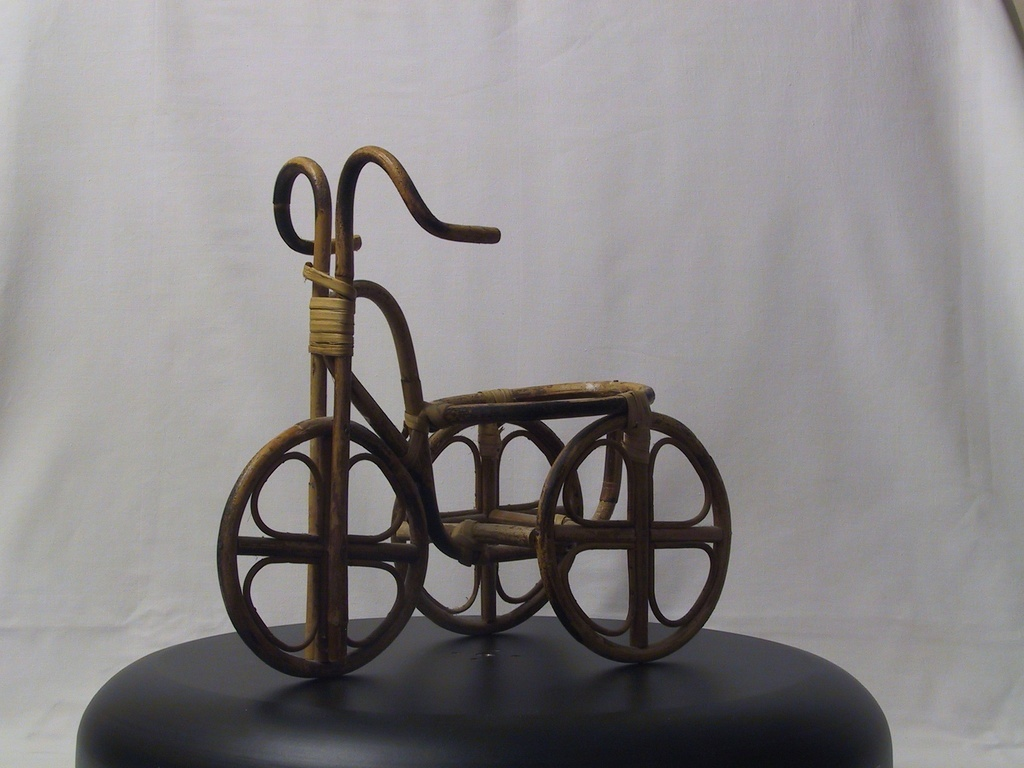
\includegraphics[width=1\columnwidth]{images/3d/15}
    \end{subfigure}%
    \vspace{1.5 mm}

    \caption{15 objects from the 3D Objects dataset by Moreels
    and Pietro \cite{moreels2007evaluation}.}
    \label{fig:3d_objects}
\end{figure}


To validate matches, Moreels and Pietro propose a method using epipolar constraints \cite[p.266]{moreels2007evaluation}, which is outlined in Figure~\ref{fig:frog}.  According to their experiments, these constraints are able to identify true correspondences with an error rate of $2\%$. We use their proposed method to generate the ground truth for the evaluation of our framework.

\begin{figure}[htb]
    \centering
    \begin{subfigure}[t]{0.22\columnwidth}
        \centering
        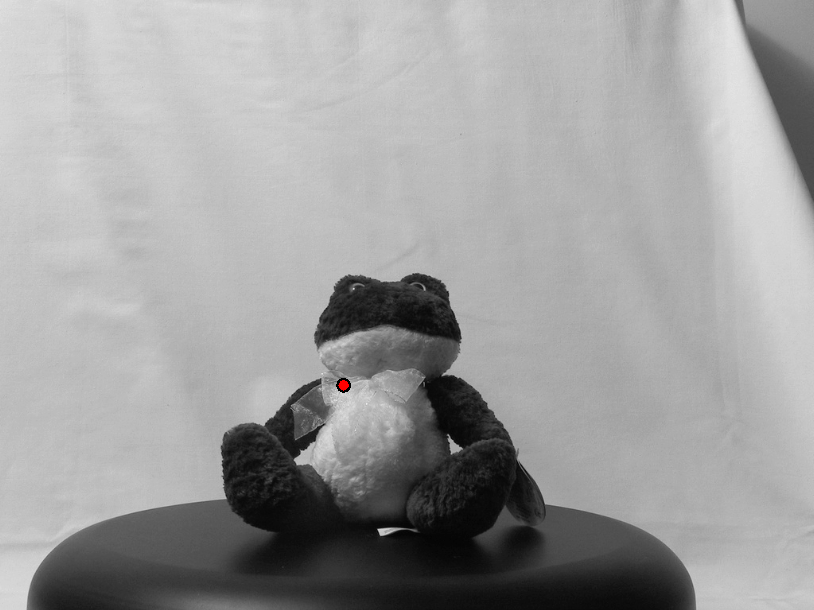
\includegraphics[width=\columnwidth]{images/Frog_A}
        \caption{Query Image}
        \label{fig:frog_a}
    \end{subfigure}%
    \quad %add desired spacing between images, e. g. ~, \quad, \qquad a 
    %blank line to force the subfigure onto a new line)
    \begin{subfigure}[t]{0.22\columnwidth}
        \centering
        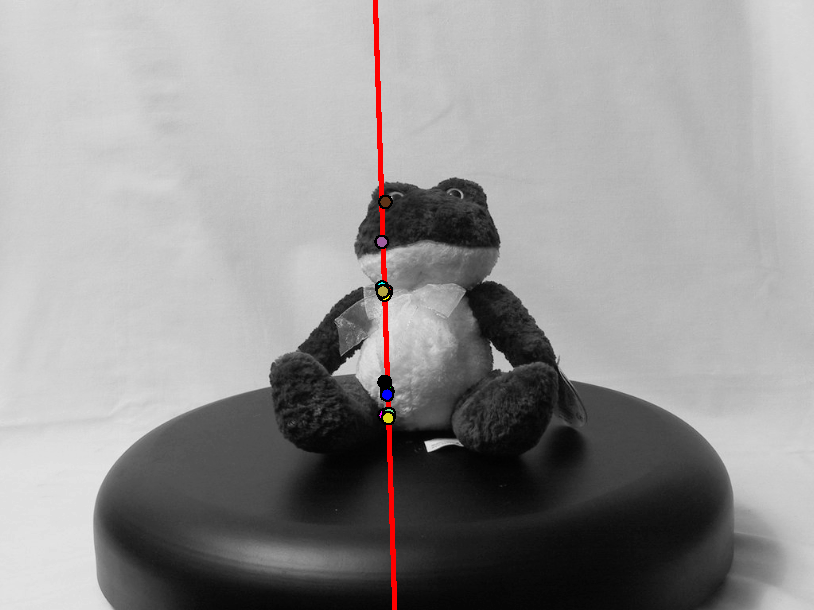
\includegraphics[width=\columnwidth]{images/Frog_B}
        \caption{Auxiliary Image}
        \label{fig:frog_b}
    \end{subfigure}%
    \quad %add desired spacing between images, e. g. ~, \quad, \qquad 
    %a blank line to force the subfigure onto a new line)
    \begin{subfigure}[t]{0.22\columnwidth}
        \centering
        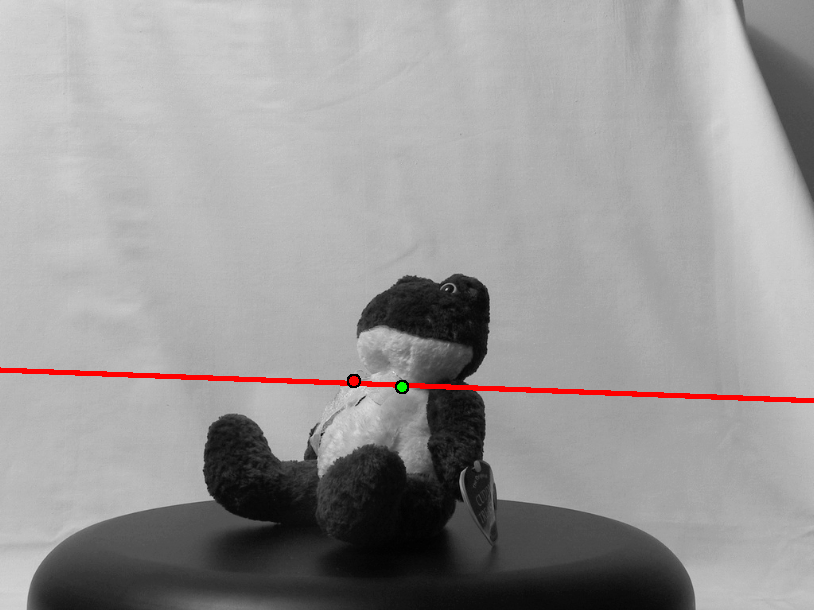
\includegraphics[width=\columnwidth]{images/Frog_C}
        \caption{Target Image}
        \label{fig:frog_c}
    \end{subfigure}%
    \quad %add desired spacing between images, e. g. ~, \quad, \qquad 
    %blank line to force the subfigure onto a new line)
    \begin{subfigure}[t]{0.22\columnwidth}
        \centering
        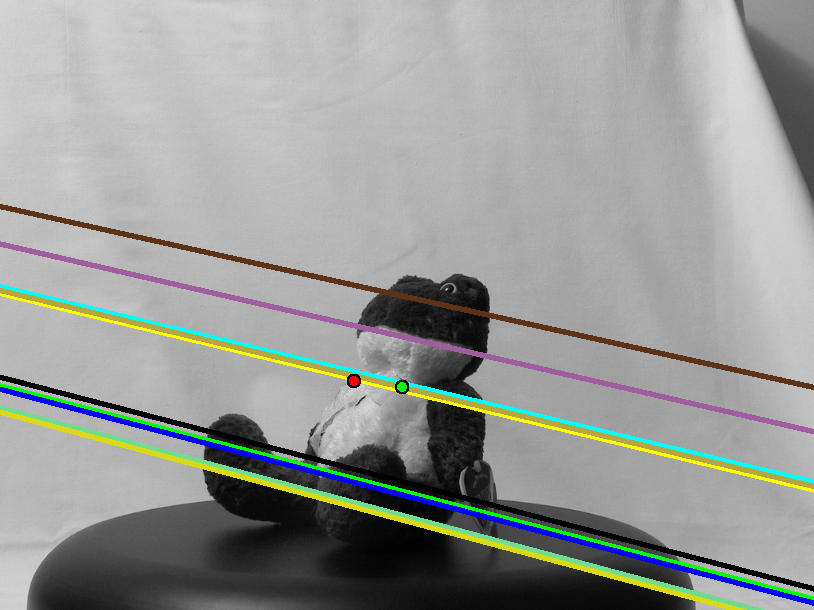
\includegraphics[width=\columnwidth]{images/Frog_C_lines}
        \caption{Target Image with epipolar constraints}
        \label{fig:frog_c_lines}
    \end{subfigure}%
    \caption{Creating epipolar constraints based on three source images \cite{moreels2007evaluation}.  (a) \emph{Query image} marked with the position of the feature we are attempting to match. (b) Auxiliary image, taken at the same rotation as the \emph{query image} but from a higher elevation angle. The line going through the image is the epipolar line of the feature point in the \emph{query image}.  The markers indicate all feature points in the image found near the epipolar line.  In c) we show the \emph{target image} which in this case is rotated 45 degrees from the \emph{query image}.  The line overlaid on the image represents the epipolar line corresponding to the feature point shown in the \emph{query image}.  The markers indicate all feature points in the image found near the epipolar line. In d) we show the \emph{target image} again, this time overlaid with the epipolar lines corresponding to all the features shown in the \emph{auxiliary image}. A true correspondence should be found within a small distance of one of the intersections of the line in c) and the lines in d). In this particular case both feature points shown in c) and d) could possibly be a correct correspondence.
}%
    \label{fig:frog}%
\end{figure}%

To compute the total number of possible correspondences, we take each feature in a \emph{query image} and count how many of them have a feature in the \emph{target image} which would satisfy the epipolar constraints outlined above. When using this dataset, features with no correspondences were not included in the set of features for testing, so as to avoid matching non-moving background and foreground objects.

We evaluate all matching algorithms from our framework on the 3D Objects dataset by matching images at different angular intervals. For each object we pick the \emph{query} image as the image taken at 10 degrees rotation for calibration stability.  We then match this image with the same object turned an additional $\Delta$ degrees, $\Delta \in \{5, 10, \ldots, 60\}$.  For every angle interval we compare images taken under 3 different lighting conditions as provided by the dataset. We include all objects in the database for which photos at 5 degree angle intervals are available except for the ``Rooster'' and ``Sponge'' objects due to image irregularities. 

\begin{figure*}[t]
	\centering
    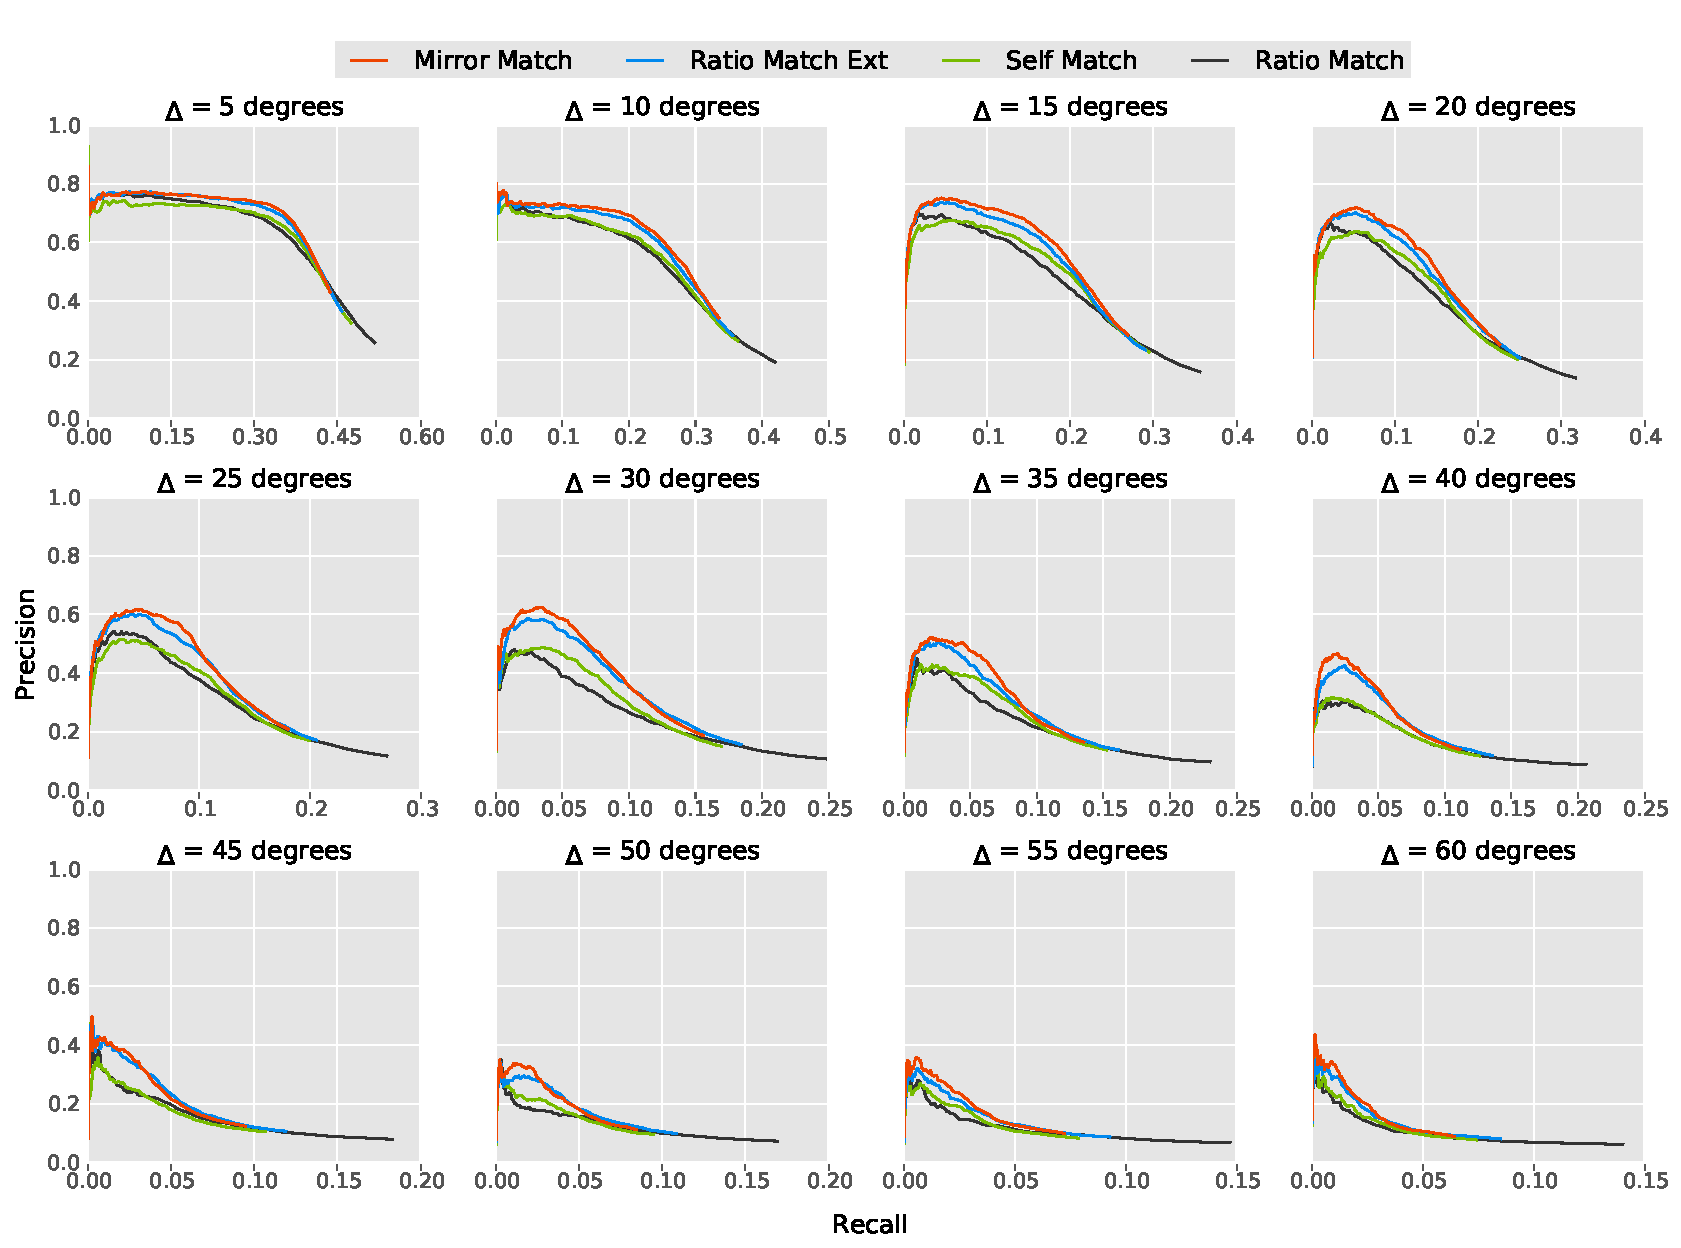
\includegraphics[width=\columnwidth]{images/results_all_objects}
    \caption{Results for the 3D objects dataset. Each plot 
    contains data accumulated from 84 objects photographed under 3 
different lighting conditions.}
    \label{fig:all_objects}
\end{figure*}

Figure~\ref{fig:all_objects} shows the performance of the different matching methods in our proposed framework for $12$ increasingly bigger angle differences. The results are shown in a precision / recall plot to make it easy to compare performance in terms of precision at similar levels of recall.  For each plot we show the accumulated results on all 3D objects, weighted by the number of possible true correspondences for the particular object. This ensures that each object contributes equally to the final result, despite some objects resulting in disproportionally more matches than others.

\emph{Ratio-Match} and \emph{Self-Match} show similar results, while \emph{Mirror-Match} and \emph{Ratio-Match-Ext} outperform both of them, showing the advantage of composing the \emph{proposed set} of features from both images. \emph{Mirror-Match} fares slightly but consistently better than \emph{Ratio-Match-Ext}. In general we see the largest performance improvements at lower recall and a  convergence of precision at higher recall. This is expected since a higher recall is a direct consequence of a more lenient threshold; as we let the threshold approach $1$, we lose the benefits of thresholding on the \emph{uniqueness ratio}, and all methods start approximating the results of a simple nearest neighbor match. For all but \emph{Ratio-Match}, the features with better matches within the same image are still weeded out, which explains the tail end of \emph{Ratio-Match} at high recall where the other algorithms no longer have results. As we demonstrated in \cite{arnfred2013mirror}, the removal of within-image matches improves performance on image pairs with partial or no overlap. For no overlap we would expect a matching algorithm to reject matches within regions that have no matching counterparts in the other image.

The performance gap between methods increases gradually with angle, reaching its maximum between $25$ and $40$ degrees, where \emph{Mirror-Match} exhibits about 20 percentage-points higher precision than \emph{Ratio-Match}. At larger viewpoint differences above $45$ degrees, the performance gain decreases.  We suspect this is partly because assumption \#2 stops being valid when the images are transformed beyond a certain level of recognizability.

To summarize, the methods perform as predicted on the 3D Objects dataset with \emph{Mirror-Match} in general performing better than \emph{Ratio-Match-Ext}, which in turn outperforms \emph{Ratio-Match}. The experimental results also show that \emph{Self-Match} overall performs equal to or better than \emph{Ratio-Match}.

\subsection{Evaluation of Descriptors}
\label{label:desc}

\begin{figure*}[t]
    \centering
    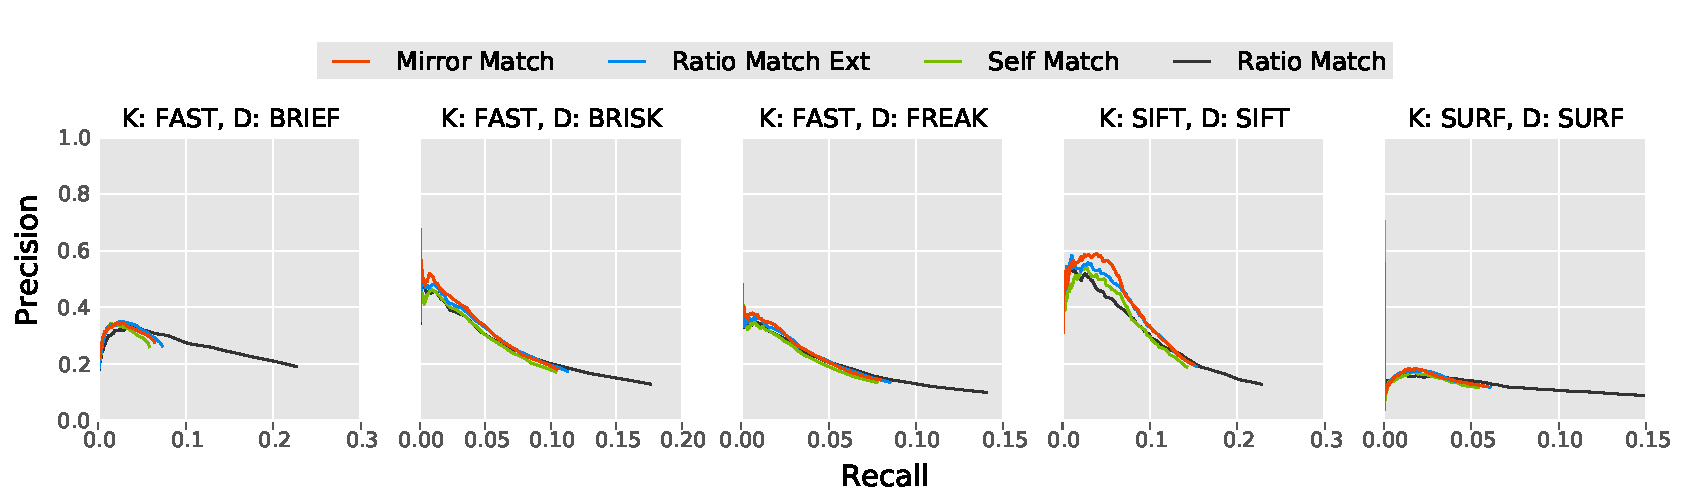
\includegraphics[width=\columnwidth]{images/results_descriptors_imageset1}
    \caption{Keypoint / Descriptor combinations measured on 15 pairs of 
    photos of 3D objects taken 25 degrees apart.}
    \label{fig:descriptors}
\end{figure*}

To evaluate whether the improvement gains with the SIFT descriptor translate to other feature descriptors such as SURF \cite{bay2006surf} or binary features such as BRIEF \cite{calonder2010brief}, BRISK \cite{leutenegger2011brisk}, or FREAK \cite{alahi2012freak}, we evaluated the different descriptors on the 3D objects data set.  The binary features were each paired with the FAST feature detector for consistency, while SIFT and SURF were tested with their respective feature detectors.  For each keypoint detector and feature descriptor pair we used the standard implementation from OpenCV 2.4.6.

The descriptors were evaluated on the 15 images  of the 3D Objects dataset pictured in Figure~\ref{fig:3d_objects}, with a fixed angle offset of 25 degrees.  Otherwise the evaluation is performed in the same manner as the general evaluation of 3D Objects in Section~\ref{S:3dobjects}, and the data presented is accumulated over the 15 objects, each set of results weighted by the possible number of correspondences.

The results in Figure~\ref{fig:descriptors} are again in line with the theoretical performance analysis of Section~\ref{S:Proofs}. They also show a clear difference in the variance of matching method performance between SIFT and the rest of the descriptors. The performance of \emph{Mirror-Match} using SIFT shows a clear increase in precision over \emph{Ratio-Match} at equal recall levels. For other descriptors the improvement is much less pronounced.  For SURF, BRISK, and BRIEF we see a small improvement in precision using \emph{Mirror-Match} over \emph{Ratio-Match} and \emph{Ratio-Match-ext}, whereas FREAK yields similar results no matter what algorithm is used.  For all descriptors \emph{Self-Match} performs on par with \emph{Ratio-Match}.

Part of this difference between SIFT and the other descriptors can be explained by looking at the recall rate with for example SURF\@. Given the same amount of possible matches, \emph{Ratio-Match} with SURF spans a larger range of recall.  Since all other methods filter out matches that are better matched within the same image, but show no increase in precision, we can conclude that correct matches are discarded because there are better matches within the same image. This violates assumption \#2 stating that a descriptor is well behaved and matches best with a descriptor of a true correspondence. This means that for this particular evaluation case, SURF and the binary features tested are not sufficiently discriminative to provide a viable case for preferring \emph{Mirror-Match} over \emph{Ratio-Match}.

\subsection{Computational Performance}

In terms of computational complexity, the algorithms can be implemented in $O(n\log n)$, if we assume that both the \emph{query} and the \emph{target} image have $n$ feature points. For a \emph{target image} with $m$ features where $m$ is significantly different from $n$, the complexities are as noted in Table~\ref{table:running_times}. In practice the constant factors involved in the actual matching of two images with approximately the same number of feature points are usually small enough that all the algorithms run at very similar speeds. This is also shown in Table~\ref{table:running_times}, which contains the running times as measured while matching 15 3D objects under three different lighting conditions ($42$ image pairs were matched in total). The running times are averaged over three separate runs of each algorithm implemented using the same data structures and libraries in Python. 

\begin{table}[htb]
\caption{Complexity and running times tested on 45 image pairs with average $n = 237$ and average $m = 247$ feature points
as tested on a Intel\textregistered\ Core\texttrademark\ i5-3550 CPU @ 
3.30~GHz with 8~GB memory.}
\label{table:running_times}
	\centering
%	\small
    \begin{tabular}{{l}{l}{l}}
    Algorithm & Complexity & Running Time\\
    \hline
    \noalign{\smallskip}
    %
    \emph{Self-Match} & $O(n\log(nm))$ & 118s  \\
    %\emph{Self-Match-Ext} & $O(n\log(n(n+m)))$ & 109s\\
    \emph{Ratio-Match} & $O(n\log(m))$ & 114s\\
    \emph{Ratio-Match-Ext} & $O(n\log(n+m))$ & 112s\\
    %\emph{Both-Match} & $O(n\log(n(n+m)))$ & 116s\\
    \emph{Mirror-Match} & $O(n\log(n+m))$ & 110s \\
    \hline
\end{tabular}
\end{table}

\subsection{Extending to Multiple target images}
%
When we match a \emph{query image} against multiple \emph{target images}, as for example in image stitching, assumption \#1 that any feature in the \emph{query image} has at most one real correspondence in the set of target features is no longer true. It might be the case that two \emph{target images} contain the same real object which yields two target features that are both real correspondences. In this case calculating the \emph{uniqueness ratio} by dividing the distance of one real correspondence with the distance to another renders it entirely useless if the two features are found in sets where there might be more than one correct correspondence.

Brown et al.\ \cite{brown2005multi} propose calculating the uniqueness ratio by taking the average of the $n$ nearest neighbors in each of the $n$ \emph{target images}. Since their particular case deals with images that are aligned horizontally one after the other, this approach is not flawed per se. However for the more general case of $N$ \emph{target images} with an unknown amount of overlap in the target group, their approach would not work since several features in the target group could possibly be a correct correspondence. 

This leaves us with two alternatives. Either we match the \emph{query image} to every \emph{target image} individually, or we use a matching strategy where the \emph{baseline set} is guaranteed not to contain any real correspondences. \emph{Self-Match} provides such a set, since the \emph{baseline set} of \emph{Self-Match} only contains features in the \emph{query image} itself. All the other methods discussed use the \emph{target image} to construct the \emph{baseline set}, which means that a baseline match might very well be a correct correspondence, leading to a \emph{uniqueness ratio} close to $1$. In addition, matching a \emph{query image} to $N$ \emph{target images} with \emph{Self-Match} is vastly faster than matching the \emph{query image} to every \emph{target image}: If we assume that every of the $N$ images has $n$ features, then matching the \emph{query image} to all $N$ images can be done in $O(Nn\log(n))$ using a metric tree. However, matching with \emph{Self-Match} is done in $O(n\log(nN)) = O(n\log(N) + n\log(n))$.

\section{Conclusions}
\label{S:Summary}

We have proposed a framework of matching methods building on the ideas behind \emph{Ratio-Match} and \emph{Mirror-Match} introducing the variations \emph{Self-Match} and \emph{Ratio-Match-Ext}. We formally proved under three assumptions that \emph{Mirror-Match} performs better than or equal to \emph{Ratio-Match-Ext} in terms of precision and recall, which in turn performs better than or equal to \emph{Ratio-Match}.

From an evaluation using images of rotated 3D objects, we have shown that the theoretical conclusions are confirmed by our experimental evaluation, with \emph{Mirror-Match} often outperforming \emph{Ratio-Match} significantly over 3024 image pairs. Finally we show that the theoretical conclusions hold across a variety of popular feature descriptors (SIFT, SURF, BRISK, BRIEF, and FREAK). These performance gains come for free in terms of both computational complexity as well as actual computing time.

With the framework we introduced three simple methods that are all applicable in situations where \emph{Ratio-Match} is currently used.  \emph{Ratio-Match-Ext} and \emph{Mirror-Match} can readily and easily replace \emph{Ratio-Match} without any performance penalty and with an increase in precision.  However, both are limited to matching image pairs like \emph{Ratio-Match}. \emph{Self-Match} on the other hand, which is on par with \emph{Ratio-Match} across all evaluations, can be applied when matching multiple overlapping images. 

\appendix

\section{Proof of equivalence of Self-Match and Self-Match-Ext}
\label{A:self}

In this appendix we prove the equivalence between \emph{Self-Match} and \emph{Self-Match-Ext}. To do this, we look at the nearest neighbor $f_{nn}$ of every query feature $f_{q}$ and consider the two cases of $f_{nn} \in F_{q}$ and $f_{nn} \in F_{t}$. For $f_{nn} \in F_{t}$ the uniqueness ratio of \emph{Self-Match-Ext} is:
\begin{align*}
    r &= \text{r}(f_{q}, F_{p}, F_{b}) \\
        &= \text{r}(f_{q}, F_{q} \cup F_{t}, F_{b})\\
        &= \text{r}(f_{q}, F_{t}, F_{b})
\end{align*}

Since $F_{p} = F_{t}$ for \emph{Self-Match} this shows that when the nearest neighbor is found in the \emph{target image}, the two algorithms behave identically. For $f_{nn} \in F_{q}$ we know that the best match for the query feature is in the \emph{query image} itself. Since neither algorithm returns a correspondence within the same image, they also behave identically for this case. This proves that for any set of \emph{query features} \emph{Self-Match} returns the same matches as \emph{Self-Match-Ext}.

\section{Proof of equivalence of Both-Match and Mirror-Match}
\label{A:mirror}

In this appendix we prove the equivalence between \emph{Both-Match} and \emph{Mirror-Match}. This proof is almost identical to the equivalence proof between \emph{Self-Match} and \emph{Self-Match-Ext}. To prove the equivalence, we look at the nearest neighbor $f_{nn}$ of every query feature $f_{q}$ and consider the two cases of $f_{nn} \in F_{q}$ and $f_{nn} \in F_{t}$. For $f_{nn} \in F_{t}$ the uniqueness ratio of \emph{Mirror-Match} is:
\begin{align*}
    r &= \text{r}(f_{q}, F_{p}, F_{b}) \\
        &= \text{r}(f_{q}, F_{q} \cup F_{t}, F_{b})\\
        &= \text{r}(f_{q}, F_{t}, F_{b})
\end{align*}

Since $F_{p} = F_{t}$ for \emph{Both-Match} this shows that when the nearest neighbor is found in the \emph{target image}, the two algorithms behave identically. For $f_{nn} \in F_{q}$ we know that the best match for the query feature is in the \emph{query image} itself. Since neither algorithm returns a correspondence within the same image, they also behave identically for this case. This proves that for any set of \emph{query features} \emph{Both-Match} returns the same matches as \emph{Mirror-Match}.

\balance

\section*{References}
\bibliographystyle{elsarticle-num}
\bibliography{bibliography}
\end{document}
